% !TeX root = ../thuthesis-example.tex

\chapter{基于最优控制理论的触摸运动模型}\label{section:model}

最优控制理论是数学最优化的分支,研究使动力控制系统的性能指标实现最优化的综合方法。自1962年Pontryagin等人提出最优控制理论以来\cite{kopp1962pontryagin},该理论被广泛应用于空间技术\cite{lewis2012optimal}、运筹学\cite{ross2020optimal}、经济调控\cite{kamien2012dynamic, ross2016nonsmooth}等重要领域。1985年,Flash等人指出,最优控制理论还可用于描述人的手部运动过程:人在组织手部运动时,大脑不会具体地控制肩关节和肘关节的旋转角度,而是将注意力集中在手掌,试图在规定时间内,最平稳地将手部从初始点移动到目标点。其中,“最平稳地”指的是人下意识地最小化手了部运动急动度平方的积分:

\begin{equation}
	min\int_{0}^{t_1}\left(\left(\frac{d^3x}{dt^3}\right)^2+\left(\frac{d^3y}{dt^3}\right)^2+\left(\frac{d^3z}{dt^3}\right)^2\right)dt
	\label{equ:objective_function}
\end{equation}

其中,$x(t)$,$y(t)$和$z(t)$是手部位置在直角坐标系三个轴上的分量随时间变化的函数。受到这份工作的启发,本文作者通过实验验证发现,公式\ref{equ:objective_function}约束下的运动方程同时也是触摸运动的良好拟合。因此,本文提出了基于最优控制理论的触摸运动模型。本章分四小节介绍触摸运动模型:

\begin{enumerate}
\item \textbf{触摸运动模型的数学表达}:提出描述触摸运动的数学方程,描述触摸运动中手指位移与时间之间的关系。
\item \textbf{触摸运动模型的计算方法}:提出利用运动传感信号拟合触摸运动方程的计算方法,其中运动传感信号包括手指的位移、速度和加速度。
\item \textbf{触摸运动模型的实验评估}:通过实验解释模型的提出过程,评测触摸运动模型的拟合精度。
\item \textbf{触摸运动模型的指导意义}:讨论触摸运动模型对几种基础触摸交互技术的指导意义,介绍模型对触摸检测、触摸意图推理和触摸手势识别的优化原理。
\end{enumerate}

%\item \textbf{模型运动模型的应用方向}:讨论触摸运动方程为触摸交互技术带来的有用信息,讨论如何利用这些信息改进触摸交互技术。

%为了方便阅读,在本章的前三节中,作者会直接给出结论,进行简单的论证。然而,部分结论需要复杂的论证过程,甚至需要通过用户实验验证,其验证过程将留在第四小节(模型的提出过程和实验评估)详细介绍。

\section{触摸运动模型的数学表达}

\textbf{触摸运动模型}是描述触摸前后极短时间内手指运动规律的模型,其数学表达是触摸运动中手指位置$x$与时间$t$关系的函数。触摸运动模型的数学表达也称触摸运动方程。为简化触摸运动模型的表达和计算,手指位置$x$只考虑手指在交互表面之上的高度,而不考虑手指在交互表面上的2D坐标——如引言所述,目前触摸交互技术的瓶颈在于普适性、响应性和意图性,而不在于2D坐标的精准性。触摸运动方程在时间轴上的起点是人产生触摸意图的瞬间$t=0$,结束点是人在心理上认为的触摸动作结束的时间$t=t_1$,这段时间内包含了手指接触交互表面的瞬间$t=t_c$($0<t_c<t_1$)。一般情况下触摸运动的时长$t_1$介于100毫秒到300毫秒之间。

%值得注意的是,在手指触摸到交互表面时($t=t_c$),手指由于交互表面的阻挡而停止运动,但触摸运动在人的心理上还未结束。直到再过一段短暂时间后($t=t_1$),人才会反应过来,开始组织下一轮手指运动,如抬起手指、拖拽等等。

\begin{figure}
	\centering
	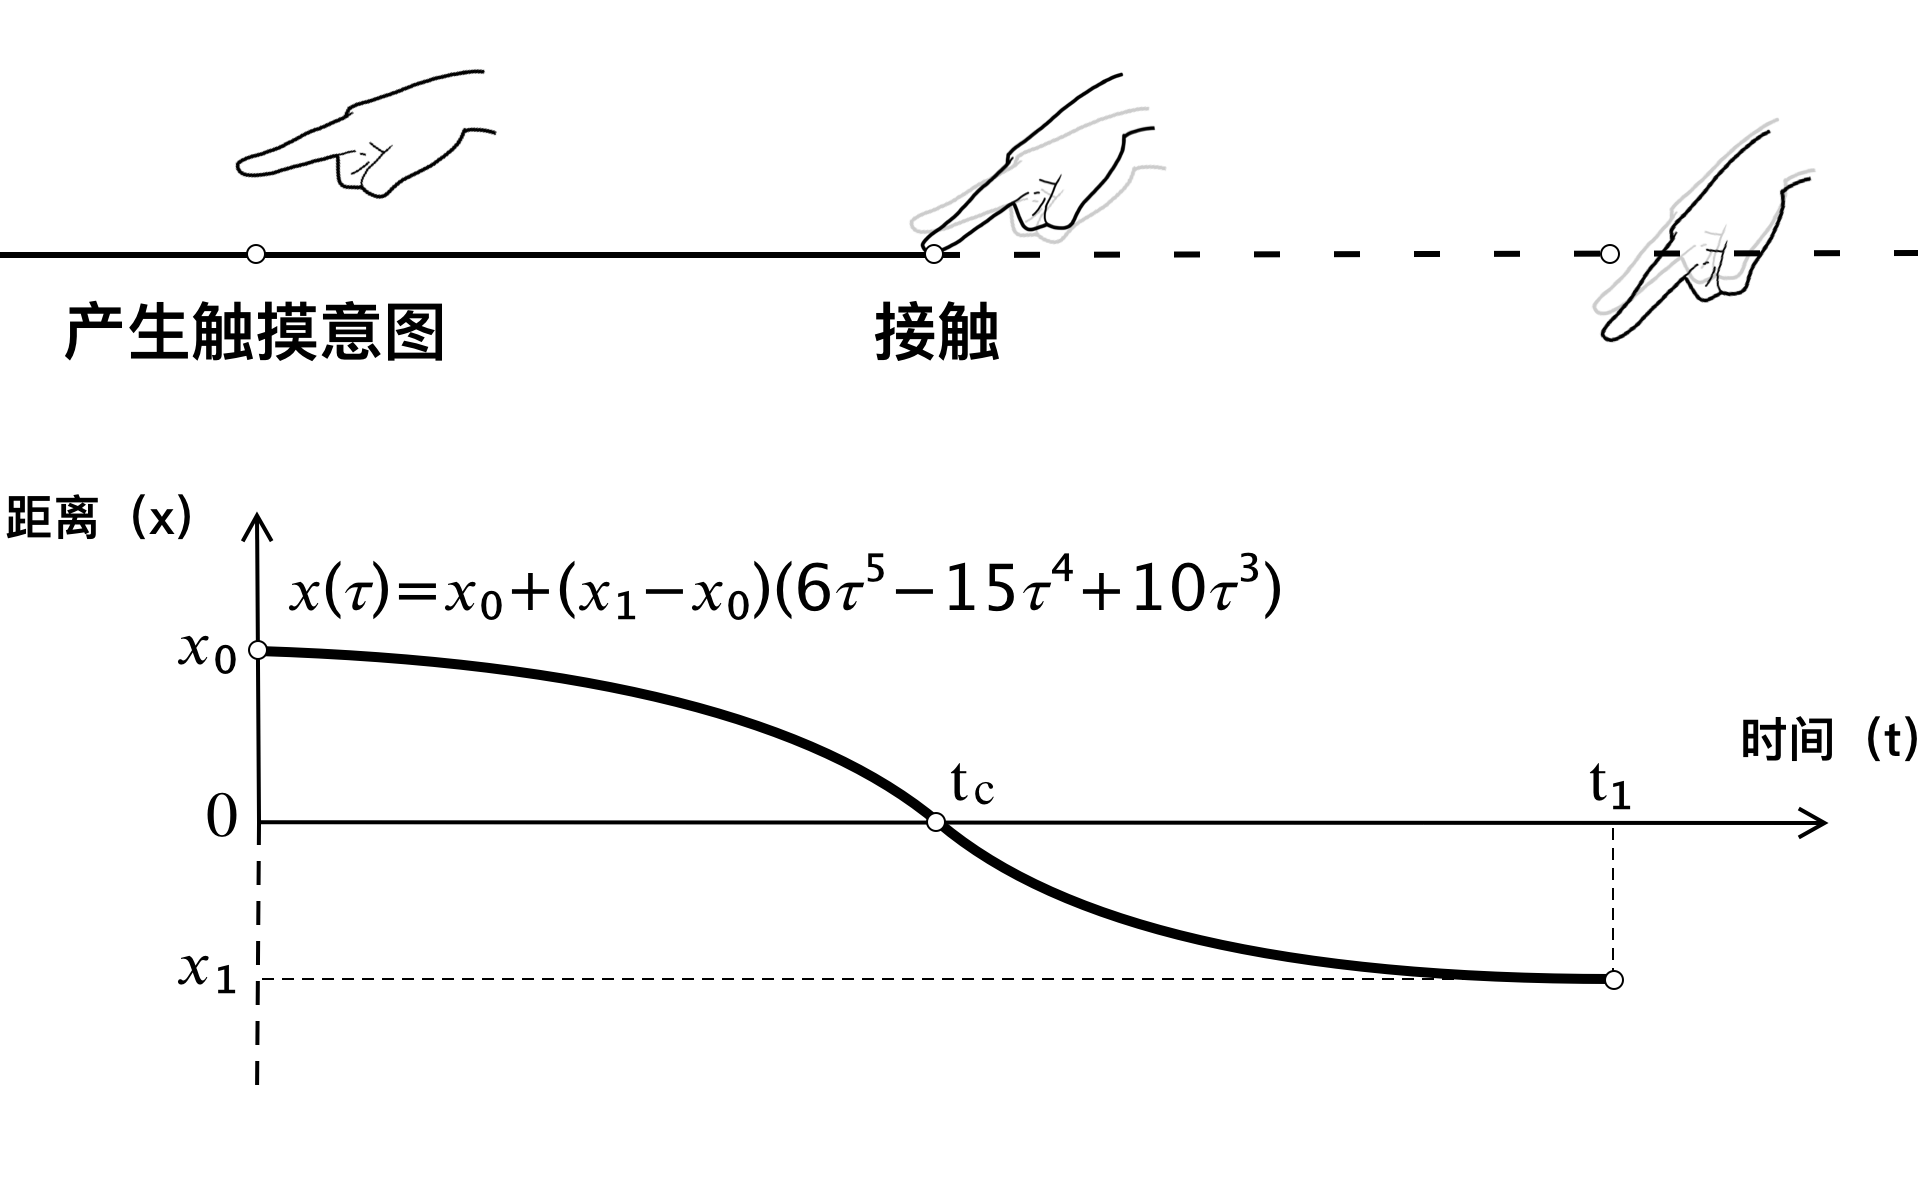
\includegraphics[width=0.8\linewidth]{touch_model_virtual.png}
	\caption*{人组织一次触摸时,假设交互表面凭空消失,人会在规定时间$t_1$内,最平稳的将手指从初始点$x_0$移动到目标点$x_1$,其时空运动轨迹如图中的公式所示。}
	\caption{无约束运动模型}
	\label{fig:touch_model_virtual}
\end{figure}

% 其中,目标点有$x_1<0$,这说明人在组织一次触摸运动时,其心理模型并非将手指刚好带到交互表面上,而是将手指带到交互表面之下的一个虚构点上

为方便理解,此处引入入\textbf{无约束运动模型},该模型基于如图\ref{fig:touch_model_virtual}所示的假想情形:“\emph{若在触摸瞬间交互表面凭空消失,人会在规定时间$t_1$内,最平稳地将手指从初始点$x_0$移动到目标点$x_1$}”。其中,“最平稳地”指的是最优控制理论对肢体运动的约束(公式\ref{equ:objective_function}),在此约束下解得无约束运动模型的数学表达为:

\begin{equation}
	x(\tau)=x_0+(x_1-x_0)(6\tau^5-15\tau^4+10\tau^3)
	\label{equ:touch_model_unconstrained}
\end{equation}

其中,$\tau=\frac{t}{t1}$是触摸运动时间进度。上述公式中$x_0>0$是容易理解的,即人在产生触摸意图时手指位于交互表面的上方。但值得注意的是,公式中有$x_1<0$,其含义是:“\emph{人在组织一次触摸运动时,其心理并非将手指带到交互表面上,而是将手指带到交互表面之下的一个虚构点上}”。

\begin{figure}
	\centering
	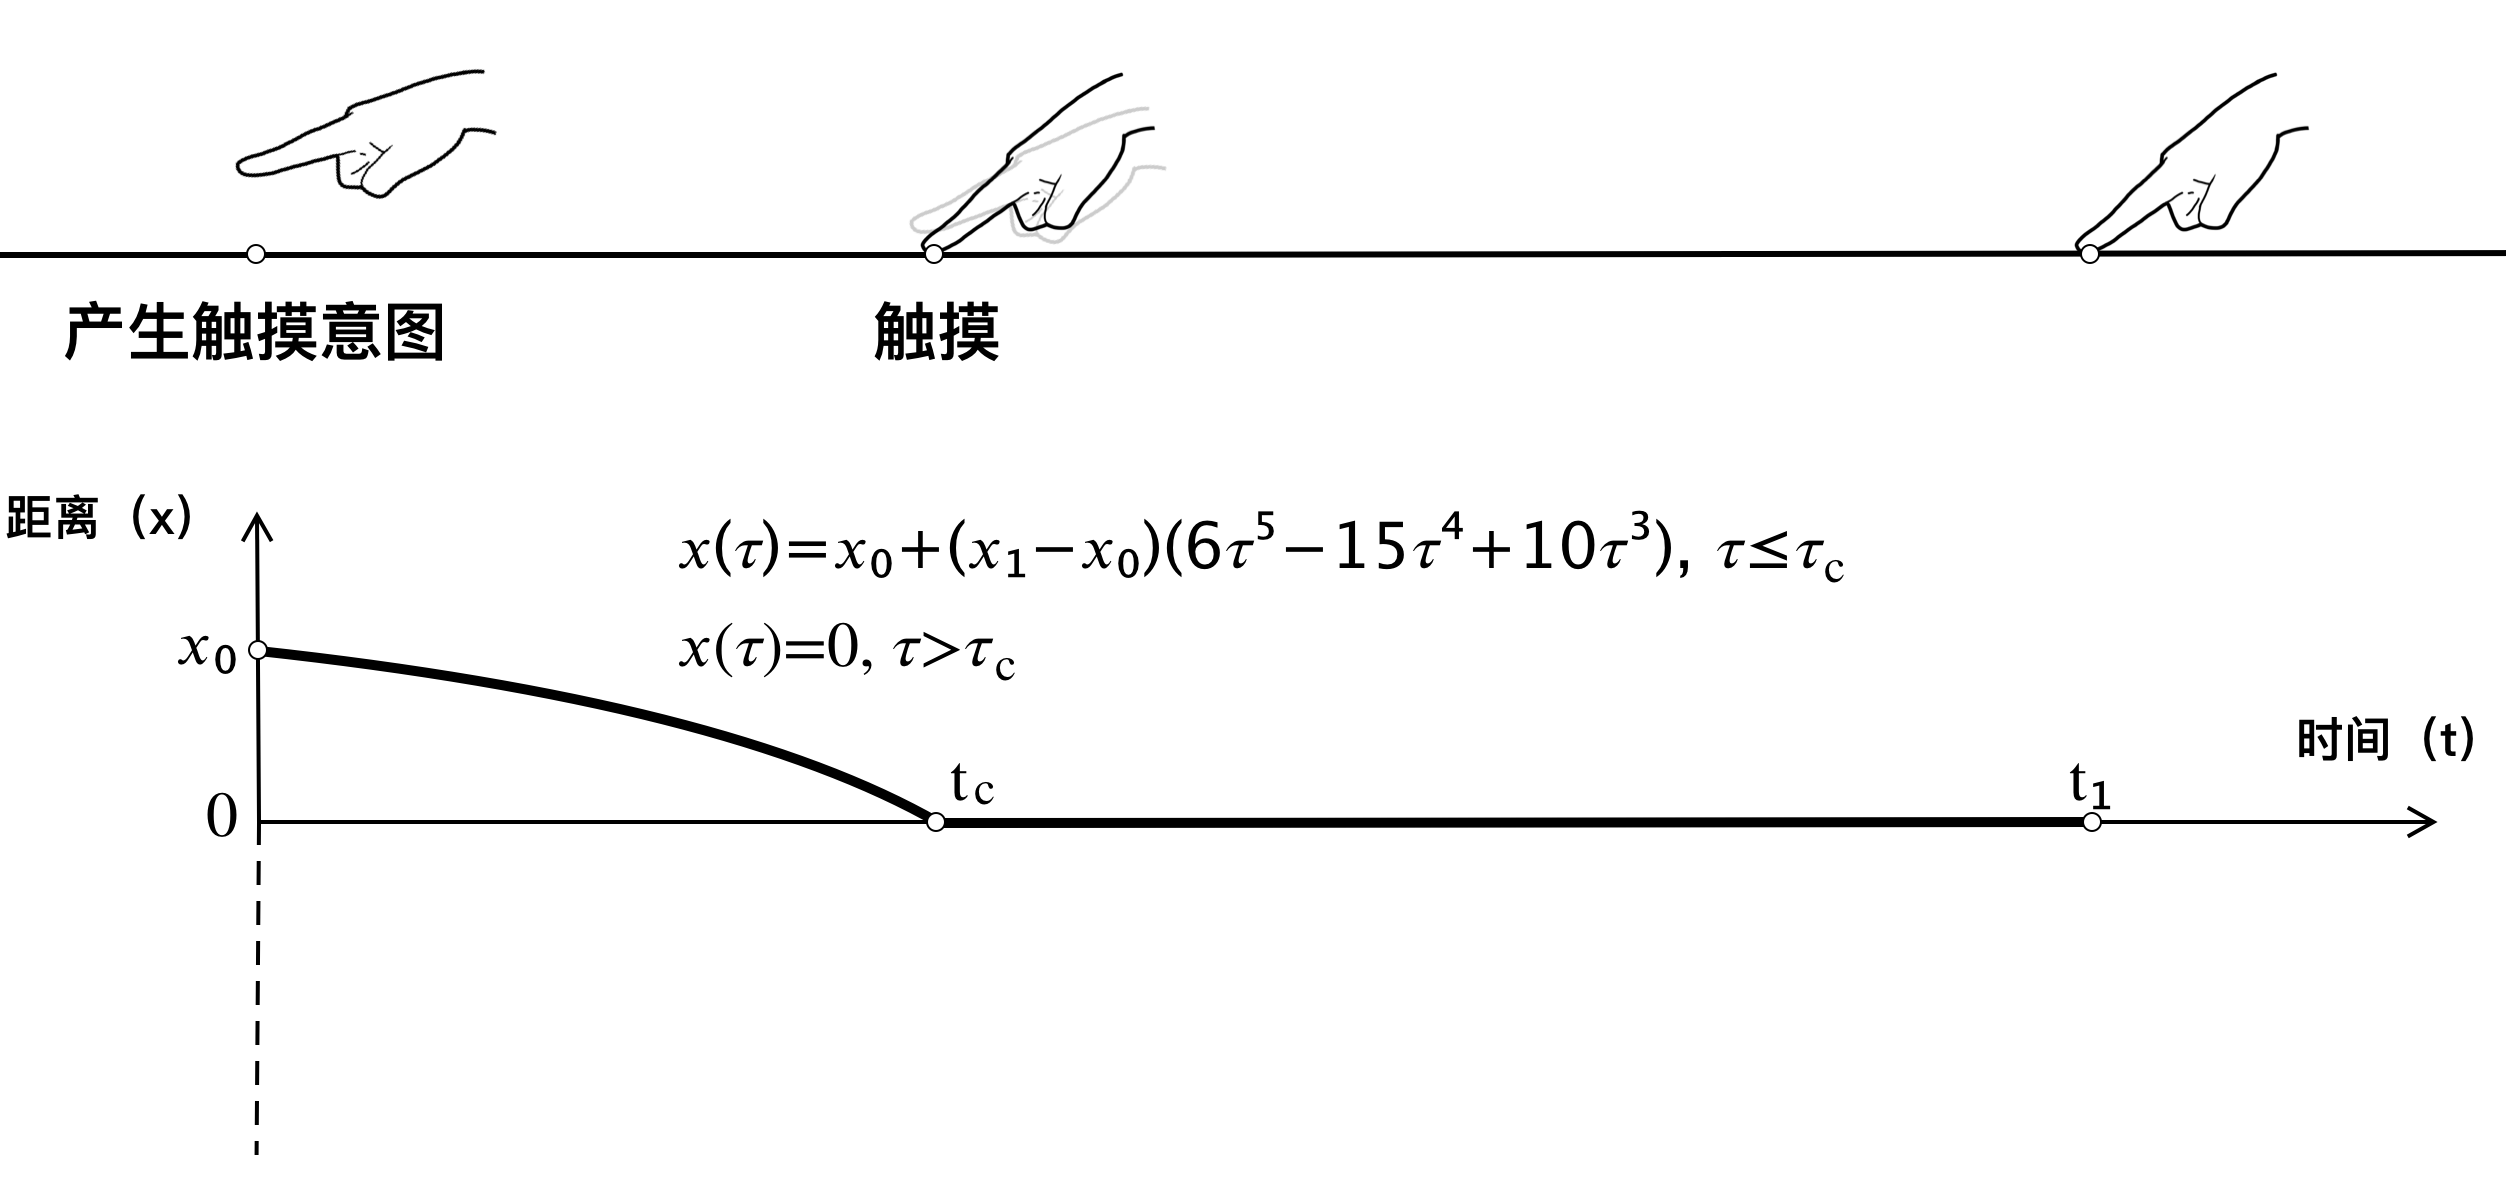
\includegraphics[width=0.8\linewidth]{touch_model_real.png}
	\caption*{一次触摸运动中,人的心理是在规定时间$t_1$内,最平稳的将手指从初始点$x_0$移动到目标点$x_1$,但交互表面的阻挡使得手指瞬间停止。触摸运动的时空运动轨迹如图中的公式所示。}
	\caption{触摸运动模型}
	\label{fig:touch_model_real}
\end{figure}

然而,如图\ref{fig:touch_model_real}所示,在实际情况下,交互表面的存在中断了上述运动过程,手指在接触到交互表面时瞬间停止了。在手指接触到交互表面之前($t<t_c$),手指运动的时空轨迹与无约束运动模型(公式\ref{equ:touch_model_unconstrained})一致;而在手指接触到交互表面之后($t>t_c$),手指静止在交互表面上。因此,\textbf{触摸运动模型}的表达式应为下述分段函数:

\begin{equation}
	x(\tau)=
	\begin{cases}
		x_0+(x_1-x_0)(6\tau^5-15\tau^4+10\tau^3)& \tau\leq\tau_c \\
		0& \tau>\tau_c
	\end{cases}
	\label{equ:touch_model}
\end{equation}

通过函数对时间进度$\tau$的求导不难发现,触摸运动模型同时揭示了手指速度$v$和加速度$a$的变化规律:

\begin{equation}
v(\tau)=
\begin{cases}
	(x_1-x_0)(30\tau^4-60\tau^3+30\tau^2)& \tau<\tau_c \\
	0& \tau>\tau_c
\end{cases}
\label{equ:touch_model_v}
\end{equation}

\begin{equation}
	a(\tau)=
	\begin{cases}
		(x_1-x_0)(120\tau^3-180\tau^2+60\tau)& \tau<\tau_c \\
		0& \tau>\tau_c
	\end{cases}
\label{equ:touch_model_a}
\end{equation}

综合以上三个公式中可以看出,触摸运动过程分为两部分,前半部分中手指处于一个向下运动的过程,其运动的时空轨迹较为复杂,是本节讨论的重点;后半部分手指静止在交互表面上,手指的位移、速度和加速度恒为零。本节的剩余内容主要讨论触摸运动方程的前半部分,也就是触摸运动的向下过程。

\subsection{单位触摸运动方程}

描述一次触摸运动的向下过程只需要三个参数,分别是$x_0$、$x_1$和$t_1$。其中,$x_0$是人产生触摸意图时手指的位置,$x_1$是人组织这次触摸运动时假想的目标点,$t_1$是人组织触摸运动时假想的运动时长。触摸运动轨迹的拟合过程,就是求解$x_0$、$x_1$和$t_1$的过程。

\begin{figure}
	\centering
	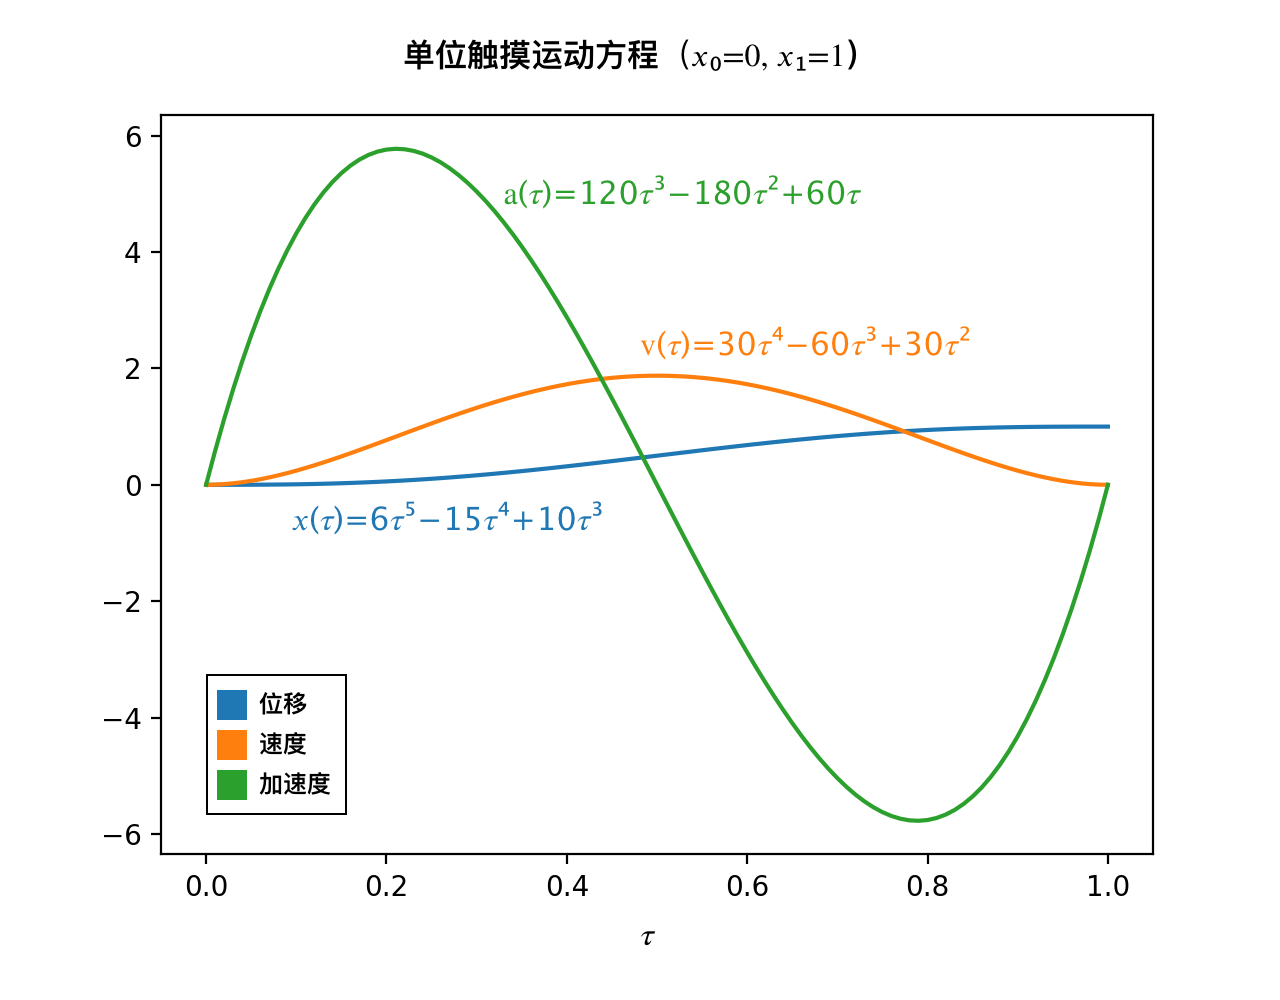
\includegraphics[width=0.8\linewidth]{std_curve.png}
	\caption*{单位触摸运动方程是归一化的触摸运动时空轨迹,其位移、速度和加速度的轨迹如图所示。}
	\caption{单位触摸运动方程}
	\label{fig:std_curve}
\end{figure}

如图\ref{fig:std_curve}所示是单位触摸运动方程,是归一化的触摸运动时空轨迹($x_0=0,x_1=1,\tau=\frac{t}{t1}$)。由于拟合触摸运动方程只涉及$x_0$、$x_1$和$t_1$这三个参数的求解,所以任何触摸运动方程的都是单位触摸运动方程在X轴和Y轴上分别缩放和平移的结果。

\subsection{触摸运动方程的推导过程}

本小节将介绍触摸运动方程的推导过程。与许多经典模型一样(如费茨定理\cite{fitts1954information}),基于最优控制理论的触摸运动模型建立在一些必要的前提条件(假设或简化)之上,以保证模型简洁明了,这将有利于模型的计算和应用。触摸运动方程的手指向下过程有两个前提条件:

\textbf{(1)触摸运动中手指的向下运动过程符合无约束运动模型}:若交互表面凭空消失,人会在规定时间$t_1$内,将手指从初始点$x_0$移动至虚构的目标点$x_1$,且移动过程最小化了手指急动度的平方的积分(公式\ref{equ:objective_function})。

\textbf{(2)手指在初始点$x_0$和目标点$x_1$上静止}:在这两点上手指的速度和加速度为零。

前提一是一个假设,该假设来自Flash等人对手部肢体运动的建模\cite{flash1985coordination}。一方面,该假设已经在先前工作中得到了充分的验证,证明其对肢体运动的拟合良好;另一方面,在这一假设下本文提出了触摸运动方程,也良好地拟合了触摸运动的实验数据。

前提二是本文对触摸运动规律的有意简化。事实上,$x$在触摸运动的初始点和目标点上仅仅是接近于静止,而非完全静止。特别是,在初始点上手指可能有初速度;在目标点上手指可能有一个向上的加速度。尽管与事实有一定的偏差,本模型仍然保留了这一简化:一方面,该简化对拟合程度的影响较小;另一方面,该简化将触摸运动方程的未知参数限制在三个以内($x_0$、$x_1$和$t_1$),提高了模型的可计算性和实用性。综上所述,触摸运动中手指的向下运动过程等价于以下最优化问题:

\begin{equation}
	\begin{cases}
		x(t) \\
		s.t. x(0)=x_0,x^{'}(0)=x^{''}(0)=0,x(t_1)=x_1,x^{'}(t_1)=x^{''}(t_1)=0 \\
		min\frac{1}{2}\int_{0}^{t_1}\left(\frac{d^3x}{dt^3}\right)^2dt
	\end{cases}
\end{equation}

读者可能注意到,手指运动应受到人的运动能力的限制,比如,手指运动存在速度和加速度的上限。然而,上述最优化问题未包含对运动能力作出条件约束,这是因为,该最优化问题的解恰巧不会超出手部运动能力的限制。求解上述最优化问题即可得到无约束运动模型的数学表达(公式\ref{equ:touch_model_unconstrained}),结合交互表面的存在中断了手指的无约束运动,进一步可推得完整的触摸运动方程(公式\ref{equ:touch_model})。

\subsection{更复杂的触摸运动方程}\label{section:complex_model}

上一小节提到,本文的触摸运动模型经过了有意简化。那么,如果没有这些简化,是否仍能求解出触摸运动模型的数学表达呢?答案是肯定的,只不过触摸运动方程会变得复杂,不利于模型的计算和应用。本小节介绍一些更复杂的触摸运动方程。

\textbf{(1)若手指仅在初始点$x_0$上静止,而在目标点$x_1$上存在一个向上的加速度$a_1(a_1>0)$。}则触摸运动方程为,待拟合参数有$x_0$、$x_1$、$t_1$和$a_1$:

\begin{equation}
	x(\tau)=
	\begin{cases}
		x_0+(x_1-x_0)[(6+\frac{a_1}{2})\tau^5+(-15-a_1)\tau^4+(10+\frac{a_1}{2})\tau^3]& \tau\leq\tau_c \\
		0& \tau>\tau_c
	\end{cases}
	\label{equ:touch_model_a1}
\end{equation}

\textbf{(2)若手指仅在目标点$x_1$上静止,而在初始点$x_0$上存在一个初速度$v_0$。}则触摸运动方程为,待拟合参数有$x_0$、$x_1$、$t_1$和$v_0$:

\begin{equation}
	x(\tau)=
	\begin{cases}
		x_0+(x_1-x_0)[(6-3v_0)\tau^5+(-15+8v_0)\tau^4+(10-2v_0)\tau^3]& \tau\leq\tau_c \\
		0& \tau>\tau_c
	\end{cases}
	\label{equ:touch_model_v0}
\end{equation}


\section{触摸运动模型的计算方法}

触摸运动的计算方法指的是利用位移、速度、加速度等运动传感信号拟合触摸运动方程参数的计算方法。如图\ref{fig:motion_sensors}所示,常见的针对手指的运动传感方法有(1)基于视觉方法的位移传感\cite{harrison2011omnitouch, xiao2018mrtouch, paradiso2000sensor, agarwal2007high, chang2005real, letessier2004visual, sugita2008touch, grudin2001integrating, saba2012dante, xiao2016direct, benko2012miragetable, wilson2010combining, newcombe2011kinectfusion, mistry2011mouseless, xiao2013worldkit};(2)基于惯性传感器的加速度传感\cite{gu2019accurate, shi2020ready, gu2020qwertyring, meier2021tapld, lam2002mids, oh2017anywheretouch, niikura2014anywhere, liu2020keep}。由于大多数速度传感器利用位移除以时间来计算速度,相比于位移传感不提供额外的信息,因此本文不讨论速度信号。

\begin{figure}
	\centering
	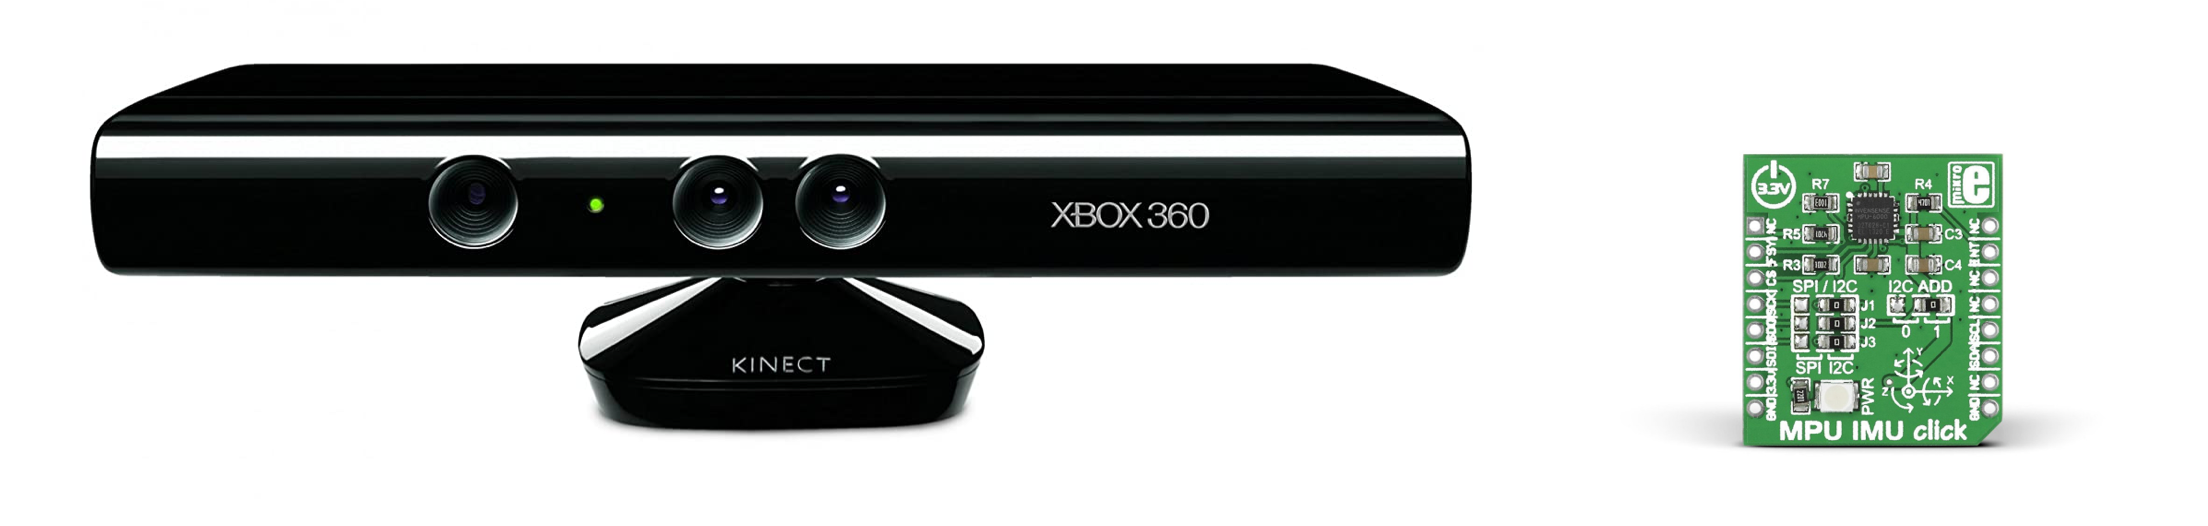
\includegraphics[width=1.0\linewidth]{motion_sensors.png}
	\caption*{左图是基于双目视觉的代表性位移传感器Kinect\cite{zhang2012microsoft},可捕捉人体四肢和手指的三维坐标;右图是惯性传感器,属于嵌入式设备,可传感自身的加速度和角速度。}
	\caption{常用的运动传感器}
	\label{fig:motion_sensors}
\end{figure}

实验观察发现,触摸运动中手指向下运动过程的时长在50毫秒到100毫秒之间。因此,触摸运动的计算应利用触摸发生前50毫秒的数据拟合触摸运动方程。假设位移传感器的采样频率为$f_x$,加速度传感器的采样频率为$f_a$,则触摸发生前50毫秒内的测量数据为:

\begin{equation}
\begin{cases}
[x_m(1), x_m(2), \cdots, x_m(N_x)]& N_x=\lfloor0.05f_x\rfloor \\
[a_m(1), a_m(2)s, \cdots, a_m(N_a)]& N_a=\lfloor0.05f_a\rfloor
\end{cases}
\end{equation}

触摸运动的计算方法可定义为利用上述测量数据拟合触摸运动方程(公式\ref{equ:touch_model})中参数$x_0$、$x_1$和的$t_1$算法,本节的剩余内容将介绍该算法。触摸运动的计算方法分为两个步骤:步骤一通过卡尔曼滤波融合各运动传感信号;步骤二通过最小二乘法拟合触摸运动方程。

\subsection{卡尔曼滤波}

在所有可能的在线滤波方法中,卡尔曼滤波对带有高斯白噪声的线性系统有着最佳的估计效果\cite{humpherys2012fresh},对于位移、速度和加速度等运动信号而言,卡尔曼滤波是很好的预处理方法。如本章所述,针对手指的运动传感方法中最常见的是位移和加速度传感,因此本小节将介绍如何利用卡尔曼滤波平滑位移信号,同时估算速度。设位移信号的误差服从正态分布$(0,\sigma_x^2)$,加速度信号的误差服从正态分布$(0,\sigma_a^2)$,设$\boldsymbol{x}=\begin{bmatrix}x&\dot{x}\end{bmatrix}^T$,则卡尔曼滤波的状态空间表达式为:

\begin{equation}
\boldsymbol{x}(k+1)=\boldsymbol{A}_d\boldsymbol{x}(k)+\boldsymbol{B}_d a_m(k)+\boldsymbol{u}
\end{equation}

\begin{equation}
x_m(k)=
\begin{bmatrix}
1 & 0
\end{bmatrix}
\boldsymbol{x}(k)+w
=\boldsymbol{H}\boldsymbol{x}(k)+w
\end{equation}

其中,$\boldsymbol{u}\sim(0,\boldsymbol{Q})$,$\boldsymbol{Q}=\begin{bmatrix}0&0\\0&\sigma_a^2\end{bmatrix}$,$w\sim(0,\sigma_x^2)$,$\boldsymbol{A}_d=\begin{bmatrix}1&T_a\\0&1\end{bmatrix}$,$\boldsymbol{B}_d=\begin{bmatrix}T_a^2/2\\Ta\end{bmatrix}$,$T_a=\frac{1}{f_a}$。算得卡尔曼滤波的协方差矩阵$\boldsymbol{Q}_d$和$\boldsymbol{R}_d$为\cite{lewis1986optimal}:

\begin{equation}
\boldsymbol{Q}_d=\sigma_a^2
\begin{bmatrix}
T_a^3/3 & T_a^2/2 \\
T_a^2/2 & T_a
\end{bmatrix}
\end{equation}

\begin{equation}
\boldsymbol{R}_d=\frac{\sigma_x^2}{T_a}
\end{equation}

由此卡尔曼滤波算法可以总结为:

\textbf{(1)时间更新:}

\begin{equation}
\boldsymbol{\hat{x}}(k+1|k)=\boldsymbol{A}_d\boldsymbol{\hat{x}}(k|k)+\boldsymbol{B}_d a_m(k)
\end{equation}

\begin{equation}
\boldsymbol{P}(k+1|k)=\boldsymbol{A}_d \boldsymbol{P}(k|k) \boldsymbol{A}_d^T+\boldsymbol{Q}_d
\end{equation}

\textbf{(2)测量更新:}

\begin{equation}
\boldsymbol{\hat{x}}(k+1|k+1)=\boldsymbol{\hat{x}}(k+1|k)+\boldsymbol{K}(k+1)[x_m(k+1)-\boldsymbol{H}\boldsymbol{\hat{x}}(k+1|k)]
\end{equation}

\begin{equation}
\boldsymbol{P}(k+1|k+1)=[\boldsymbol{I}-\boldsymbol{K}(k+1)\boldsymbol{H}]\boldsymbol{P}(k+1|k)
\end{equation}

其中,卡尔曼增益$\boldsymbol{K}(k+1)$为:

\begin{equation}
\boldsymbol{K}(k+1)=\boldsymbol{P}(k+1|k)\boldsymbol{H}^T[\boldsymbol{H}\boldsymbol{P}(k+1|k)\boldsymbol{H}^T+\boldsymbol{R}_d]^{-1}
\end{equation}

通过上述卡尔曼滤波即可估计第k帧的位移和速度$\boldsymbol{\hat{x}}(k|k)=\begin{bmatrix}x(k)&v(k)\end{bmatrix}^T$。若位移信号的采样间隔$T_d$和加速度的采样信号$T_a$不同,且$T_d/T_a=M$为整数,则在每M帧同时执行时间更新和测量更新,其余帧只执行时间更新:

\begin{equation}
\boldsymbol{\hat{x}}(k+1|k+1)=\boldsymbol{\hat{x}}(k+1|k)=\boldsymbol{A}_d\boldsymbol{\hat{x}}(k|k)+\boldsymbol{B}_d a_m(k)
\end{equation}

\begin{equation}
\boldsymbol{P}(k+1|k+1)=\boldsymbol{P}(k+1|k)=\boldsymbol{A}_d \boldsymbol{P}(k|k) \boldsymbol{A}_d^T+\boldsymbol{Q}_d
\end{equation}

\subsection{最小二乘拟合}

拟合触摸运动方程(公式\ref{equ:touch_model})的过程是求解未知量$x_0$、$x_1$和$t_1$最大似然值的过程。本节提到,拟合触摸运动方程需要用到最近50毫秒内的运动传感信号,设近50毫秒内的第一帧数据$(x_m(1),a_m(1))$对应触摸运动方程的时间戳$t_s$,即时间序列$[x_m(1), x_m(2), \cdots, x_m(N_x)]$和$[a_m(1), a_m(2)s, \cdots, a_m(N_a)]$对应触摸运动方程中$t\in [t_s,t_s+0.05]$的部分,则$t_s$也是一个需要拟合的未知量。由于传感器误触符合正态分布,应采用最小二乘法拟合触摸运动方程,即求解以下最优化问题:

\begin{equation}
\begin{cases}
x_0, x_1, t_1, t_s \\
min \frac{\Sigma^{N_x}_{k=1}{\left(x_m(k)-x(t_s+k T_x)\right)^2}}{\sigma_x^2}
+ \frac{\Sigma^{N_a}_{k=1}{\left(a_m(k)-a(t_s+k T_a)\right)^2}}{\sigma_a^2}
\end{cases}
\label{equ:touch_model_calc}
\end{equation}

在计算机算法中,求解最优化问题的方法有很多\cite{bertsekas1997nonlinear, vzilinskas2006practical, bertsimas1993simulated},本章使用的最优化算法为信赖阈方法\cite{conn2000trust},在Python的科学计算工具包Scipy中,信赖阈方法的名称是“trust-constr”。拟合时还需给未知参数设置合理的初始估计值和取值范围,以提高拟合的效率和准确性。表格\ref{tab:model_parameter_limit}展示了各未知参数的初始值估计和约束条件,其中的距离单位为米,时间单位为秒:

\begin{table}
	\centering
	\caption{拟合触摸运动方程时对未知参数的约束}
	\begin{tabular}{cccc}
		\toprule
		未知参数 & 初始值 & 下限  & 上限 \\
		\midrule
	    $x_0$ & 0.01 & $x_m(1)$ & 0.03 \\
		$x_1$ & -0.035 & -0.1 & 0 \\
		$t_1$ & 0.25 & 0.05 & 0.3 \\
		$t_s$ & 0.01 & 0 & 0.05 \\
		\bottomrule
	\end{tabular}
	\label{tab:model_parameter_limit}
\end{table}

表格中各未知参数的初始值估计和取值范围均来自对大量触摸交互事件的观测。其中,初始值估计来自大量触摸运动的均值,例如,$x_0$的初始值为0.01(米),这是因为,平均而言触摸交互发生之前人的手指在交互表面上方一厘米左右。同理,$t_1$的初始值为0.2,原因是触摸运动过程的时长约为200毫秒。表格中的上限和下限覆盖了大多数触摸交互的取值范围,例如,$x_0$的下限为$x_m(1)$,这是因为,在触摸事件发生前的50毫秒时,大部分情况下手指已经进入了向下运动的过程,因此人产生触摸意图时手指与交互表面的距离$x_0$一定不小于$x_m(1)$。

在实际应用中,若仅有位移传感信号或加速度传感信号其一,本小节介绍的计算方法也是可以运作的:只需将公式\ref{equ:touch_model_calc}中待最优化函数中传感信号缺失的项置为零即可,但拟合的准确性必然会受到影响。

\section{触摸运动模型的实验评估}

本节将介绍触摸运动模型的评估实验,实验收集了人在几种典型的触摸交互任务中手指的运动信号,其中,触摸交互任务包括单次点击、连续快速点击、滑动手势、长按和拖拽。运动信号包括基于视觉方法的手指位移信号和基于惯性传感器的手指加速度信号。除了运动信号外,实验还利用压敏触摸板收集了手指触摸之后向下的压力信号。根据上述数据,本节将讨论触摸运动模型的提出过程、评测触摸运动模型的拟合精度。

\subsection{数据采集实验}

\subsubsection{实验设计和过程}

实验者从校园中招募了12名被试,其中有4名女性,被试的年龄从19岁到25岁不等,平均年龄为23.8岁,标准差为2.27。所有的被试都是右撇子。如图\ref{fig:touch_model_exp_setting}左侧所示是本实验的设置,桌子上摆放着一块压敏触摸板,作为实验的交互表面,收集触摸的力度信息。被试的手指上被绑上了一个惯性传感器,用于收集手指的加速度信号。在触摸板的远端有一个高速双目摄像头,用于收集手指的位移信号。实验分为五个阶段,在五种不同的触摸交互任务下收集被试的触摸运动信号,交互任务包括:

\begin{figure}
	\centering
	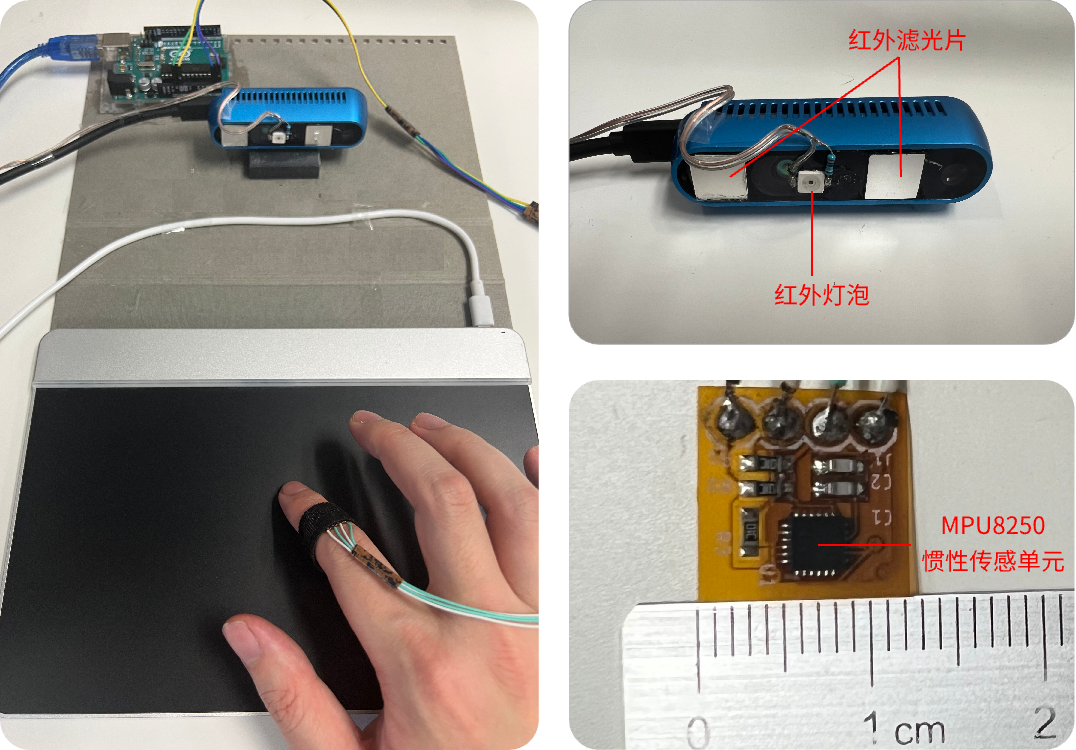
\includegraphics[width=0.8\linewidth]{touch_model_exp_setting.png}
	\caption*{左图是本实验的设置,本实验收集被试在不同的触摸交互任务下的触摸运动信号。右图是实验设备的细节。}
	\caption{触摸运动模型评估实验设置}
	\label{fig:touch_model_exp_setting}
\end{figure}

\textbf{(1)单次点击:}被试在触摸板上用食指点击50次。被试以自己喜欢的方式以任意触点位置、点击力度和角度进行触摸,但是被试需保证每两次点击之间有停顿,先将手指移动至目标触摸位置上方,瞄准之后再进行点击。实验共收集到600个单次点击数据片段。

\textbf{(2)连续快速点击:}被试在触摸板上用食指连续点击50次。在这一组实验中,为了保证被试的触摸是连续且快速的,实验者规定被试在一左一右的两个目标点上快速来回点击。实验共收集到600个连续快速点击数据片段。

\textbf{(3)滑动手势:}被试在触摸板上用食指滑动50次。被试在执行滑动手势时,想象自己在手机上做切屏动作,左滑和右滑交替进行。实验共收集到300次左滑数据和300次右滑数据。

\textbf{(4)长按手势:}被试在触摸板上用食指长按50次。被试以自己喜欢的方式以任意触点位置、触摸力度、时长和角度长按,在长按的过程中手指不可以移动,长按的时长只要求能与单次点击区分开来。被试需要保证在每次长按之前先将手指移动至目标触摸位置上方。实验共收集到600个长按数据片段。

\textbf{(5)拖拽手势:}被试在触摸板上用食指执行拖拽手势五十次。被试在执行拖拽手势时,想象触摸板上有一个手机应用图标,并将该图标左右来回拖动。实验共收集到300次向左拖拽数据和300次向右拖拽数据。

\begin{figure}
	\centering
	
\includegraphics[width=0.8\linewidth]{miss_step_exp_setting.png}
	\caption*{如左图所示,被试重复点击一个白色盒子。点击数次之后,如右图所示,实验者在被试进行下一次点击时迅速抽走盒子,高速摄像头记录这一“踏空”的触摸运动过程。}
	\caption{触摸踏空实验}
	\label{fig:miss_step_exp_setting}
\end{figure}

在每两段实验之间,被试休息一分钟的时间,以避免疲劳。数据收集实验的总时长为15分钟。在数据收集实验后,实验者还组织了一项非正式的实验,名为“触摸踏空实验”。如图\ref{fig:miss_step_exp_setting}所示,被试用食指点击一个白色盒子,实验者用高速双目摄像头捕捉被试点击盒子的过程。在被试连续点击数次之后,实验者要求被试闭上双眼并继续点击。数秒后实验者迅速移开盒子,此时被试的手指触摸运动会“踏空”,这一踏空的手指运动轨迹是触摸踏空实验采集的重点,用于验证触摸交互中手指的向下运动过程是否符合无约束运动模型(公式\ref{equ:touch_model_unconstrained})。对于每名被试,触摸踏空实验只会收集一次手指运动轨迹,这是为了避免被试知道实验意图之后,其触摸心理发生改变。

\subsubsection{实验设备}

如图\ref{fig:touch_model_exp_setting}所示是本实验的实验设备,包含一个Sensel压敏触摸板\cite{Website-Morph}、RealSense双目摄像头\cite{keselman2017intel}和一个GY-91惯性传感器。Sensel压敏触摸板是本实验的交互表面,被试在触摸板上执行触摸交互。压敏触摸板左右宽度为240毫米,上下宽度为138毫米,包含$185×105$个传感元件,间距为 1.25 毫米,每个传感单元可以感应到大约30000 个级别的压力,范围从5克到5千克不等。本实验通过压敏触摸板收集触摸的触点位置和压力随着时间变化的信号。

RealSense双目摄像头可通过自带的计算机视觉方法跟踪裸手的手指位置,但是精度不够。为了提高传感精度,实验者改装了双目摄像头,将其改装成原理类似Optitrack\cite{point2011optitrack}的针对红外反光标记点的高精度坐标跟踪系统。实验者在两个红外摄像头之间的位置上加装了一个980纳米波长的红外光灯泡,并用980纳米波长的窄通玻璃片盖住两个红外摄像头。这样一来,双目摄像头就只能看见反射红外光的物体,大大提升了图像质量。在实验中,被试在食指指甲上贴上正方形红外反射贴纸,双目摄像头可以追踪红外反射贴纸中心点的位置——红外图像中贴纸处像素为最亮的白色,通过简单的阈值方法就可以求出中心点的二维坐标,再根据双目成像原理求出手指的三维坐标,精度$\sigma_x$可达0.2毫米左右。在代码实现方面,实验者调用了RealSense的高帧率模式,帧速率为300赫兹。

商用的GY-91惯性传感器体积较大,为了将穿戴传感器对用户的影响降到最低,实验者自行设计电路图,将GY-91的核心元件MPU8250嵌入到一块宽度8毫米、厚度小于2毫米的线路板中。实验中,实验者用魔术贴将传感元件直接固定在被试的手指上,传感元件通过细长的杜邦线连接到Arduino(Uno R3)开发板上,可收集六轴的运动信号,包括三轴原始加速度和三轴角速度。其中,原始的加速度信号是线性加速度和重力混杂的结果,系统通过Madgwick滤波器\cite{madgwick2010efficient}将原始加速度分解为线性加速度和重力方向。惯性传感单元的工作频率为1000赫兹,精度$\sigma_a$为$0.5m/s^2$左右。

\subsubsection{实验数据统计}\label{section:fitting_result}

本实验共采集了$12\times5\times50=3000$次触摸的实验数据。实验者通过一个交互程序,人工剔除了明显错误的数据,例如,有的时候双目视觉追踪手指位置的算法会失败,导致手指位置信号发生跳变;有的时候由于被试的指甲太长,触摸板没有及时报告触摸事件。在剔除了错误数据之后,实验共记录了超过2800份有效的触摸交互数据。

\begin{table}
	\centering
	\caption{本实验中触摸交互数据的统计值,括号中的数值为标准差。时间单位为毫秒,距离单位为厘米,力的单位为克,速度单位为米每秒。}
	\begin{tabular}{ccccccc}
		\toprule
		统计值 & 单次点击 & 连续点击 & 长按手势  & 滑动手势 & 拖拽手势 & \textbf{总体平均} \\
		\midrule
		方程参数$x_0$ & 0.84(0.34) & 1.33(0.35) & 0.73(0.30) & 0.97(0.34) & 0.92(0.33) & \textbf{0.96(0.38)} \\
		方程参数$x_1$ & -3.89(1.50) & -3.60(1.74) & -3.19(1.55) & -4.01(1.47) & -2.90(1.72) & \textbf{-3.52(1.66)} \\
		方程参数$t_1$ & 253(60) & 246(58) & 263(58) & 271(53) & 247(64) & \textbf{256(61)} \\
		触摸时间$t_c$ & 69(11) & 79(11) & 71(13) & 76(12) & 77(13) & \textbf{75(13)} \\
		抬起时间$t_{up}$ & 176(28) & 178(29) & - & 206(51) & - & \textbf{187(41)} \\
		触摸时长$T$ & 107(28) & 99(28) & - & 130(49) & - & \textbf{112(40)} \\
		触摸速度$v(t_c)$ & 0.27(0.12) & 0.31(0.08) & 0.19(0.09) & 0.26(0.10) & 0.22(0.09) & \textbf{0.25(0.10)} \\
		力度峰值$F$ & 111(116) & 106(58) & 296(314) & 101(92) & 290(298) & \textbf{181(229)} \\
		\bottomrule
	\end{tabular}
	\label{tab:model_experiment_result}
\end{table}

如表格\ref{tab:model_experiment_result}所示是触摸交互数据的简单统计。
方程参数$x_0$指的是人产生触摸意图时手指与交互表面的距离,其均值为1厘米,即在触摸交互当中,人的非交互手指悬在交互表面上的距离大约为一厘米。
触摸时间$t_c$指的是从人产生触摸意图到手指接触交互表面所需的时间,均值为75毫秒。触摸时长$T(T=T_{up}-T_c)$指的是人的手指接触交互表面的时长,表格中只统计了短促的触摸交互的时长,均值为112毫秒。触摸速度$v(t_c)$指的是手指接触交互表面瞬间的速度,均值为0.25米每秒。力度峰值$F$指的是手指接触到交互表面以后,手指向下按压的力度的最大值,其均值为181克。统计上述数据对触摸交互技术有帮助,举例来说,在上一节——触摸运动的计算方法中,使用最优化方法拟合触摸运动方程时需要给各未知参数设置初始值和取值范围,初始值设定为表格\ref{tab:model_experiment_result}中的均值是较为合理的,而取值范围也可以根据上述实验结果来设计。

从表格\ref{tab:model_experiment_result}中还能看出,不同触摸交互任务下手指的运动轨迹也存在统计性差异。例如,若将单次点击、连续点击和滑动等归为短时触摸交互,将长按和拖住归为长时触摸交互,则这两类触摸的统计数据会有较大差异:总体来说,短时触摸交互的触摸速度$v_c$更大,假象目标点深度$x_1$更深,这一现象的原因可能是短时触摸交互更急促。接下来的三小节将利用本实验收集的数据,讨论触摸运动模型中无约束运动过程的合理性,评测触摸运动模型的拟合精度,并与先前模型进行比较。

\subsection{无约束运动模型的合理性}

本章提到,\textbf{无约束运动模型}指的是:“\emph{若在触摸瞬间交互表面凭空消失,人会在规定时间$t_1$内,最平稳地将手指从初始点$x_0$移动到目标点$x_1$}”。即人在组织一次触摸运动时,其心理并非将手指带到交互表面上,而是将手指带到交互表面之下的一个虚构点上。无约束运动模型是触摸运动模型推导过程中重要的一环,其合理性需要通过实验来求证。

% [0.43, 3.97, 2.48, 1.45, 1.96, 1.56, 0.78, 1.45, 2.21, 3.87, 3.78, 3.14]

在本实验的最后,实验者就追加了触摸踏空实验,收集了“\emph{触摸瞬间交互表面凭空消失}”时手指的运动轨迹。由于触摸踏空实验需要对被试隐瞒实验目的,每名被试只能贡献一份实验数据,数据量较少,因此此处只作非正式的定性分析:结果显示,所有被试的手指都会运动到交互表面之下,深度在0.43厘米到3.97厘米之间,平均值为2.26厘米,标准差为1.16。该结果与章节\ref{section:fitting_result}中拟合的$x1$相比更浅一些,这可能是因为真实的手指向下运动过程受到手指结构的拉扯,不是理想的无约束运动过程。尽管如此,实验结果已经表明,被试在组织一次触摸运动时,其手指运动轨迹会经过交互表面之下的一个虚构点$x_1$。

手指经过$x_1$后发生的事情因被试而异。在12名被试当中,有7名被试的手指会停在$x_1$上,这与无约束运动模型相符;而另外的5名被试的手指会在经过最低点$x_1$后折返向上,也就是说,在被试的手指达到最低点$x_1$后,手指有一个向上的加速度($a>0$),这就是章节\ref{section:complex_model}中更复杂的触摸运动方程的情形。前文已经提到,在这种情况下尽管触摸运动模型只是对实际情况的简化,但在计算上仍然是合理、高效的。

\subsection{触摸运动模型的拟合精度}

如图\ref{fig:model_fitting}所示是使用触摸运动计算模型拟合实际测量数据的两个实例,上方的两幅子图展示了一次普通力度点击的拟合效果,下方的两幅子图展示了一次较轻点击的拟合效果。左侧子图是对触摸运动位移的拟合,右侧子图是对加速度的拟合。从图中可以看出,下方触摸运动轨迹的目标点深度更浅,因此对应一次力度更轻的点击。

\begin{figure}
	\centering
	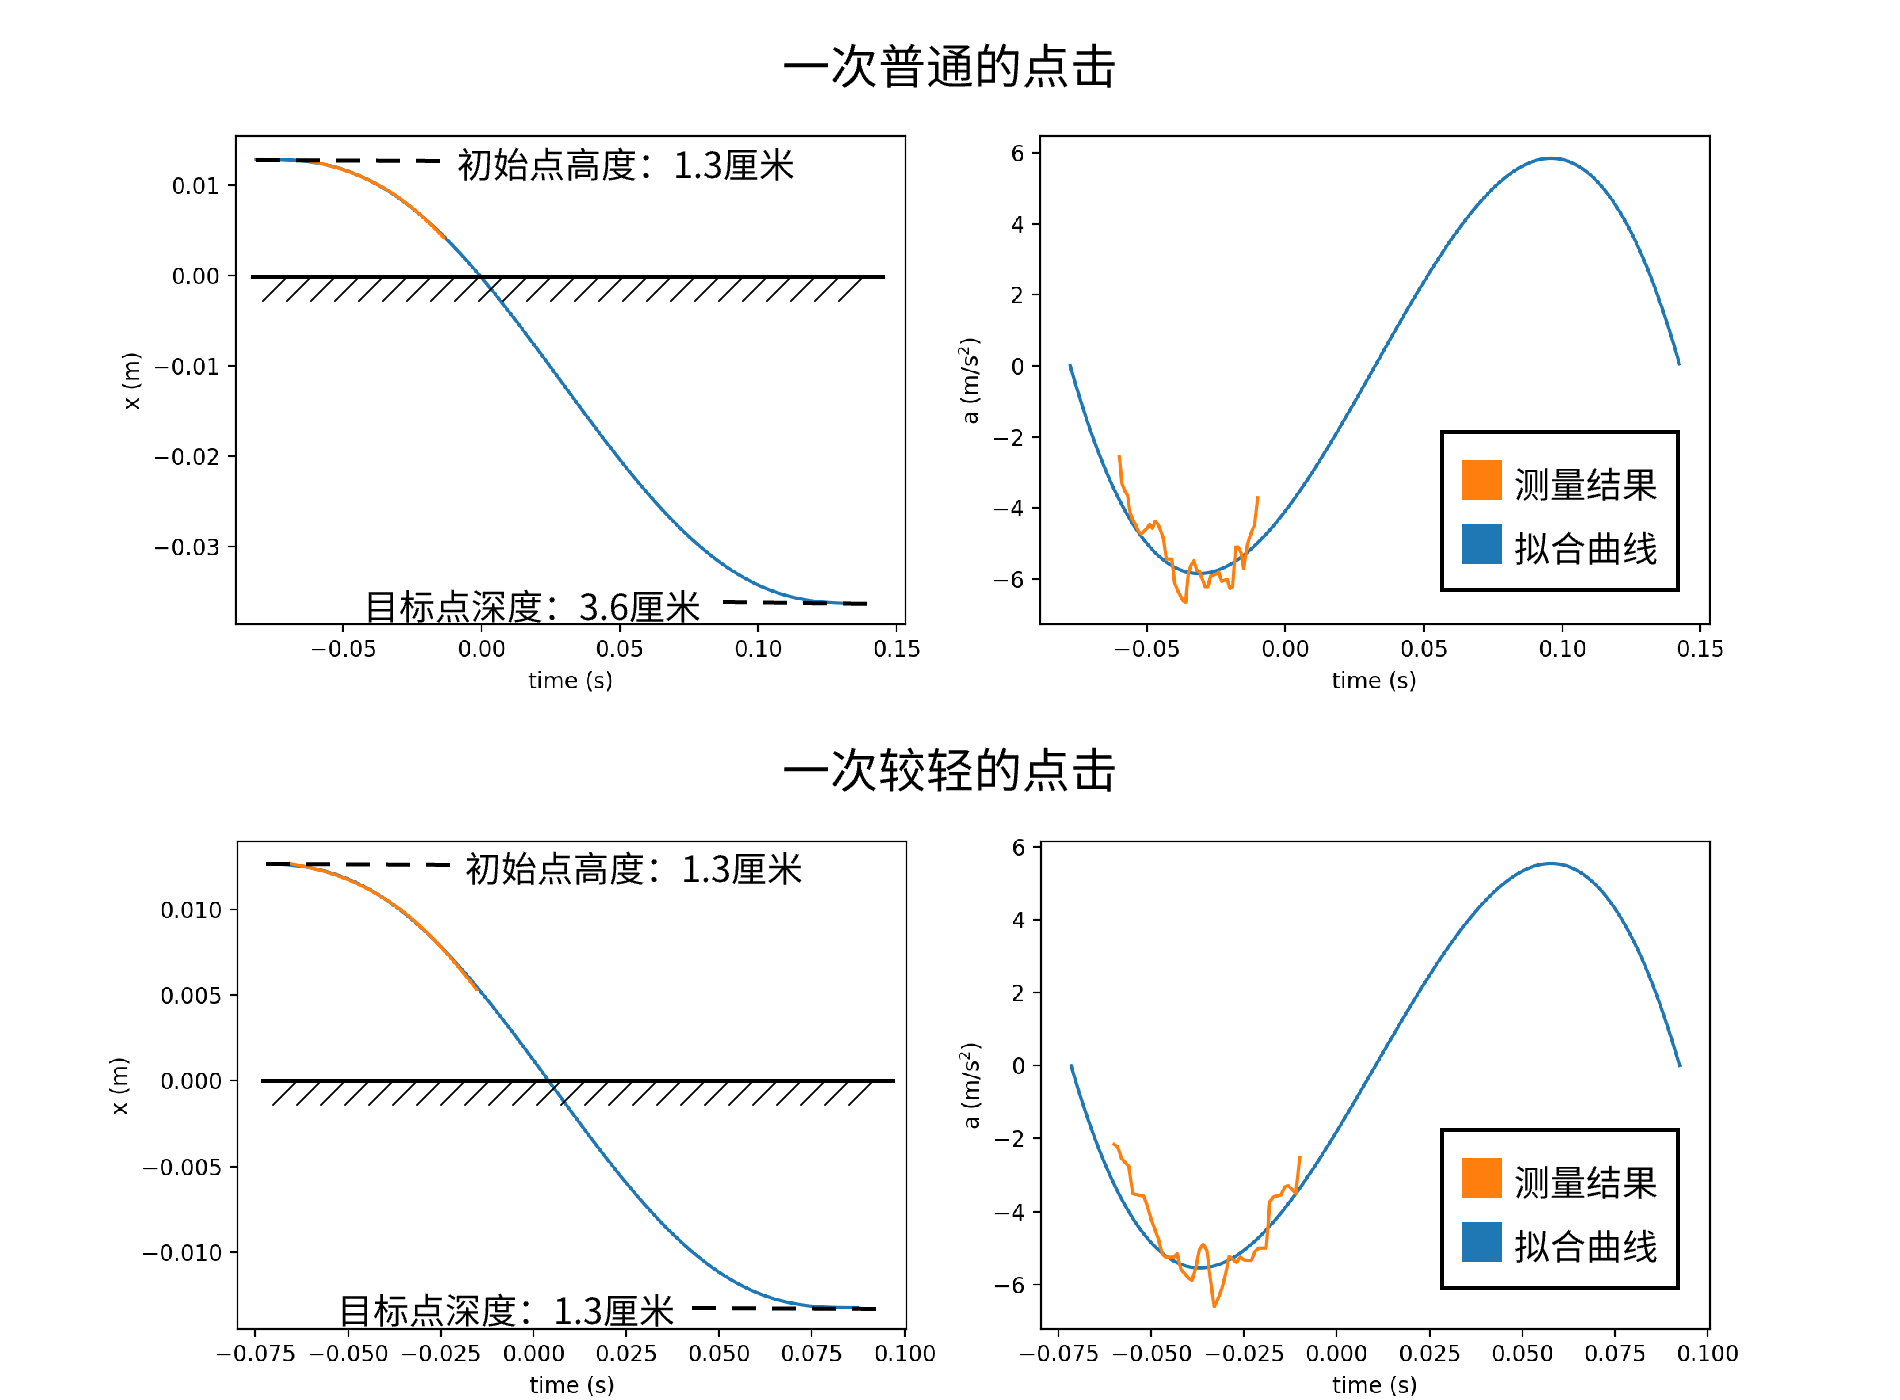
\includegraphics[width=1.0\linewidth]{model_fitting.png}
	\caption*{上方两幅子图展示了一次普通点击的位移和加速度时空曲线,下方两幅子图展示了一次较轻点击的相关曲线。从图中可以看出,拟合曲线与测量结果相符。}
	\caption{触摸运动模型的拟合实例}
	\label{fig:model_fitting}
\end{figure}

本小节通过均方根误差(RMSE)来评估触摸运动方程的拟合精度:

\begin{equation}
	RMSE(x)
	=\sqrt{\frac{1}{N_x}\Sigma^n_{k=1}{\left(x_m(k)-x(t_s+k T_x)\right)^2}}
\end{equation}

\begin{equation}
	RMSE(a)
	=\sqrt{\frac{1}{N_a}\Sigma^m_{k=1}{\left(a_m(k)-a(t_s+k T_a)\right)^2}}
\end{equation}

其中,$RMSE(x)$是触摸运动位移方程的均方根误差,$RMSE(a)$是加速度方程的均方根误差。在本实验的数据集中,$RMSE(x)=8.6\times10^{-5}m=0.086mm$,是位移传感器标准误差$\sigma_x$的43.01\%,可见触摸运动模型对触摸前50毫秒内位移信号的拟合精度非常高。$RMSE(a)=0.64m/s^2$,是惯性传感器标准误差$\sigma_a$的127.08\%。

\begin{figure}
	\centering
	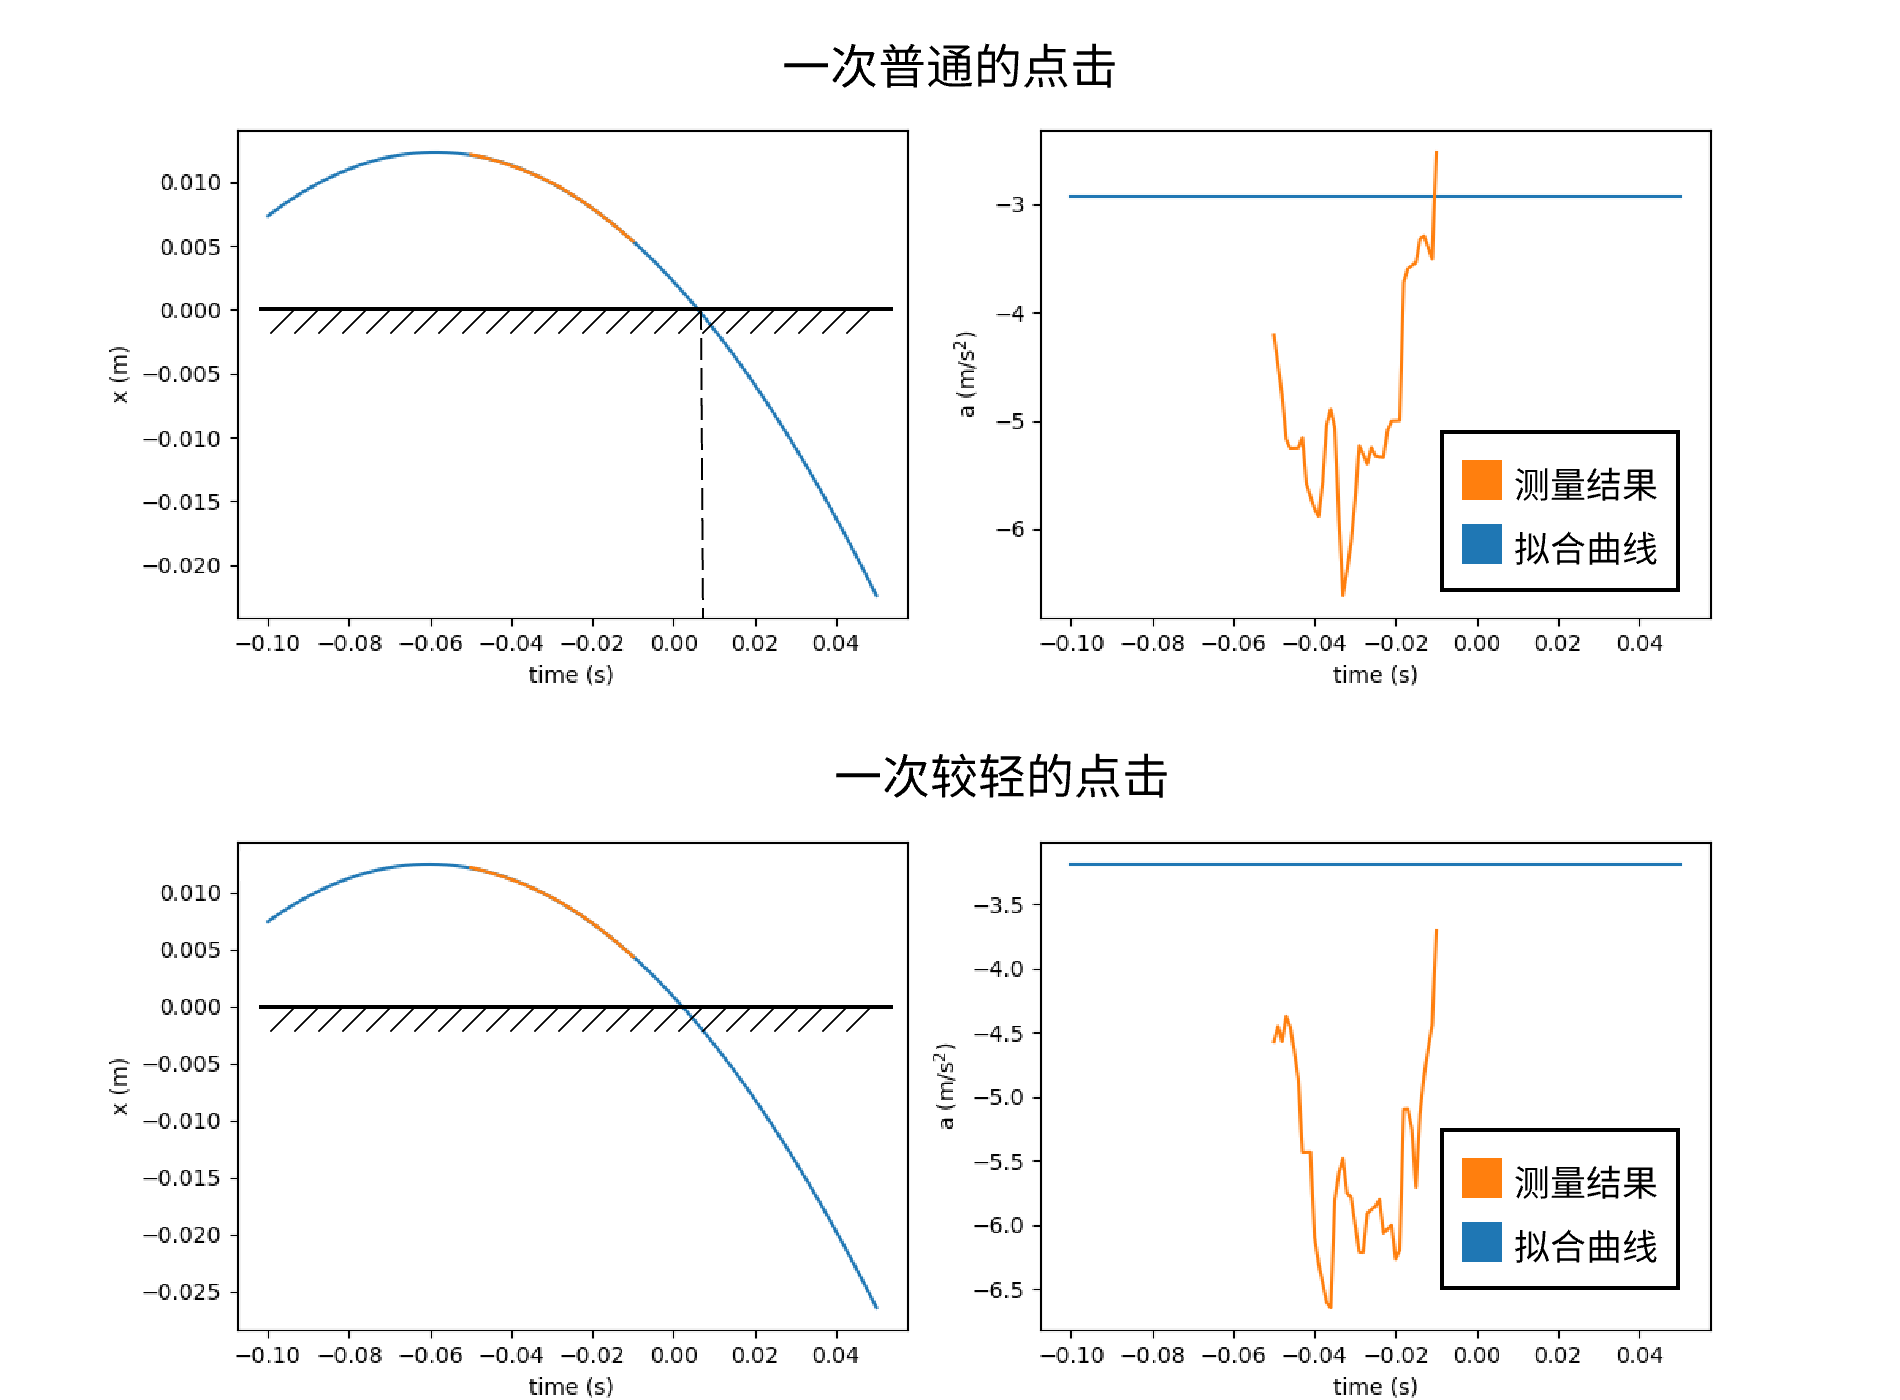
\includegraphics[width=1.0\linewidth]{parabola_fitting.png}
	\caption*{图中展示了抛物线对两次触摸实例的拟合效果。抛物线只能较好地拟合位移信号,而无法很好地拟合加速度信号,因为触摸运动过程并非匀加速运动。}
	\caption{抛物线对触摸运动的拟合实例}
	\label{fig:parabola_fitting}
\end{figure}

为了对比触摸运动模型与现有模型,本小节复现了相关工作中\cite{xia2014zero}利用抛物线拟合触摸运动的方法,该工作利用手指的空中运动轨迹预测触摸事件发生的时间,以抵消系统延迟带来的影响。如图\ref{fig:parabola_fitting}所示,抛物线能较好地拟合位移信号,其中$RMSE(x)=3.5\times10^{-5}m=0.035mm$,是位移传感器标准误差$\sigma_x$的17.53\%。但是,抛物线无法很好地拟合加速度信号,其中$RMSE(a)=2.98m/s^2$,是惯性传感器标准差的597.22\%。这是因为,触摸运动过程并不是匀加速运动,相关工作中利用抛物线拟合触摸运动的方法是不符合原理的。相比之下,本文所提出的触摸运动模型能更好地预测触摸交互中的各项参数,例如触摸时间$t_c$、触摸速度$v(t_c)$等,能为触摸交互优化技术带来更大的启发。

\section{触摸运动模型的指导意义}

触摸运动模型对触摸交互技术的优化具有指导意义,本文在两种典型的触摸交互任务下评测模型对技术的优化效果:

\begin{itemize}
\item \textbf{触摸指点任务:}触摸指点任务是人通过触摸交互在图形用户界面中点中目标的任务,是触摸图形用户界面中最基础的交互任务。
\item \textbf{文本输入任务:}触摸文本输入任务是人通过连续触摸点击进行打字的任务,是最复杂、最快速的触摸交互任务。
\end{itemize}

\begin{table}
	\centering
	\caption{触摸运动模型与第\ref{section:TappingRing}、\ref{section:QwertyRing}、\ref{section:TypeBoard}章所述触摸交互技术之间的联系。}
	\begin{tabular}{|l|p{12em}|p{12em}|}
		\toprule
		 & \textbf{触摸指点任务} & \textbf{文本输入任务} \\
		\midrule
		\textbf{触摸检测} & 第\ref{section:TappingRing}章,指环上的高准确低延迟触摸检测技术 & \\
		\textbf{触摸手势识别} & & 第\ref{section:QwertyRing}章,指环上的触摸手势识别和打字技术 \\
		\textbf{触摸意图推理} & & 第\ref{section:TypeBoard}章,平板电脑上的意图推理键盘 \\
		\bottomrule
	\end{tabular}
	\label{tab:model_paper_relationship}
\end{table}

如表格\ref{tab:model_paper_relationship}所示,本文的第\ref{section:TappingRing}、\ref{section:QwertyRing}、\ref{section:TypeBoard}章将介绍三项具体的触摸交互优化技术,以验证触摸运动模型在不同触摸交互技术和交互任务下的表现。本节将从理论的角度出发,讨论触摸运动模型对触摸检测、触摸手势识别和触摸意图推理技术的指导意义,而第\ref{section:TappingRing}、\ref{section:QwertyRing}、\ref{section:TypeBoard}章将详细介绍技术的实施方案。

\subsection{触摸检测}

\textbf{触摸检测}是触摸交互中检测手指接触交互表面瞬间的技术,是检测触摸交互是否发生的技术。触摸检测的响应性是重要改进方向,即触摸检测的准确率应大于99\%,延迟应低于20毫秒,以满足人对触摸交互的感官需求\cite{jota2013fast}。

\begin{figure}
	\centering
	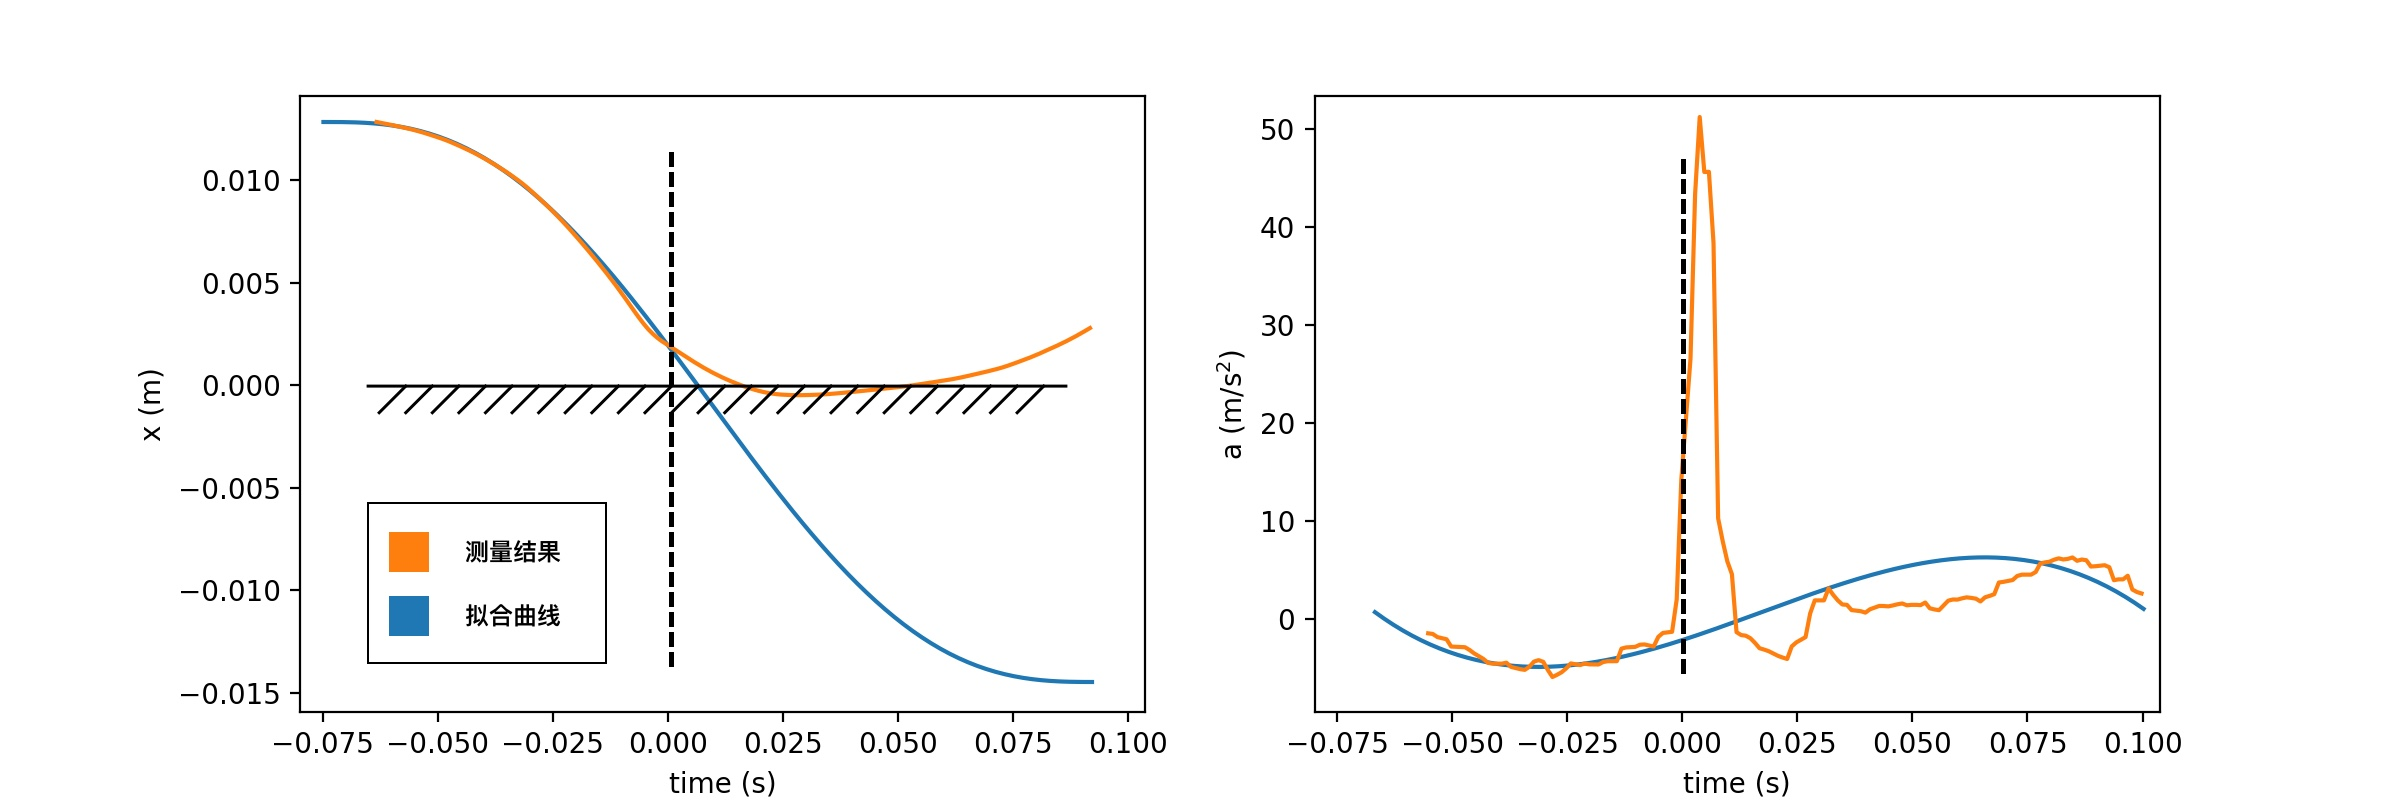
\includegraphics[width=1.0\linewidth]{illustrate_touch_sensing.jpg}
	\caption*{左图为一次触摸的位移时空轨迹,右图为加速度轨迹,黑色虚线是手指接触交互表面的瞬间,橙线是传感器的测量结果,蓝线是用手指接触之前的信号拟合的触摸运动方程。}
	\caption{模型为触摸检测提供判断依据}
	\label{fig:illustrate_touch_sensing}
\end{figure}

触摸运动模型为触摸检测技术提供了\emph{完整的判断依据}。如图\ref{fig:illustrate_touch_sensing}所示,触摸运动模型揭示,触摸由手指的向下运动过程和手指瞬停构成。在手指接触交互表面之前,手指处于向下运动过程,其轨迹符合触摸运动方程(公式\ref{equ:touch_model});在手指接触交互表面的瞬间,手指由于受到交互表面的阻碍而瞬停,使得手指位移和加速度的测量结果都大幅偏离触摸运动方程的预测结果。以位移信号为例,当传感器测量结果与触摸运动方程相差超过三倍标准差时,可以判定触摸已经发生:

\begin{equation}
	\lvert x_m(\tau_{now})-x(\tau_{now})\rvert>3\sigma_x
	\label{equ:touch_condition_intro}
\end{equation}

其中,$\tau_{now}$是当前时刻,$x(\tau_{now})$是模型预测的手指位置,而$x_m(\tau_{now})$是传感器测量结果,$\sigma_x$是将信号误差和拟合误差考虑在内的标准误差。从式子可以看出,上述判据的理论准确率为三倍标准差所对应的99.7\%。更重要的是,在保障检测准确率的前提下,利用上述式子检测触摸的延迟是理论最低的,因为在这一时刻之前,运动信号所携带的信息不足以区分“触摸已发生”和“误差导致的结果”。因此,触摸运动模型也揭示了,触摸检测的准确性和延迟优化并非独立的优化问题,而是此消彼长的关系。触摸运动模型可以在两者的动态平衡中找到最有益于交互体验的解,本文将在章节\ref{section:model_TappingRing}中结合人的触摸行为数据,详细介绍触摸检测技术。

%本文的后续分析表明,触摸交互的准确性和延迟优化并非独立的优化问题,而是此消彼长的关系:当一个触摸检测系统允许有更长的识别延迟时,它能用于检测触摸的信息就更丰富,准确率的上限就越高;但相应地,过长的识别延迟会直接影响到人的触摸交互体验。因此,触摸检测的准确性和延迟优化是需要权衡的问题,而触摸运动模型可以在两者的动态平衡中找到最有益于交互体验的解。

%触摸运动模型揭示:(1)在手指接触交互表面之前,手指会有一个向下运动过程,其时空轨迹符合触摸运动方程(公式\ref{equ:touch_model});(2)在手指接触交互表面的瞬间,手指的向下运动由于受到交互表面的阻碍而瞬停,使得手指的位移和加速度信号大幅度偏离触摸运动方程的预测结果。因此,“手指在向下运动后瞬停”是本文模型为触摸检测技术提供的判断依据。如图\ref{fig:illustrate_touch_sensing}所示是一次触摸前后的手指运动规律,左图是手指位移的时空轨迹,右图是加速度信号的时空轨迹。其中,黑色虚线是手指接触交互表面的瞬间,橙色线是信号的测量值,利用手指接触交互表面之前的数据可以拟合出触摸运动方程(蓝线)。从图中可以看出,在触摸发生之前,蓝线是橙线的良好拟合;但在触摸发生以后,橙线就和蓝线就分开了。以左图的位移信号为例,本文模型下触摸检测的判断依据可以被形式化地描述为:

%其中,$\tau_{now}$是当前时刻在触摸运动过程中的时间进度,$x(\tau_{now})$是触摸运动方程预测的手指位置,这两个值可以根据触摸运动模型的计算方法求得,而$x_m(\tau_{now})$是传感器实测的手指位置。上述式子的含义是,当传感器测得的手指位置与触摸运动方程预测结果相差超过传感器的三倍标准误差时,可以判定触摸已经发生。在位移传感器的识别误差服从正态分布的前提下,上述判据的理论准确率为三倍标准差所对应的99.7\%的置信概率。由此可见,本文模型为触摸检测技术提供的判据是十分强力的,为验证其实际有效性,本章将基于这一判据,实现一种指环上的高准确低延迟触摸检测技术。

\subsection{触摸手势识别}

\textbf{触摸手势识别}是识别并分类触摸交互手势的技术,常见的触摸手势有点击、长按、滑动、拖拽等等。触摸手势识别的难点是高准确、低延迟地检测触摸和抬起,其中,\textbf{抬起检测}指的是手指接触交互表面后,检测手指离开交互表面瞬间的技术。在准确检测触摸和抬起以后,其它触摸手势的识别往往能通过简单的阈值方法解决,例如,长按手势等价于触摸和抬起之间的时间间隔超过一定阈值;左滑手势等价于从触摸到抬起的这段时间内手指向左移动超过一定阈值。

\begin{figure}
	\centering
	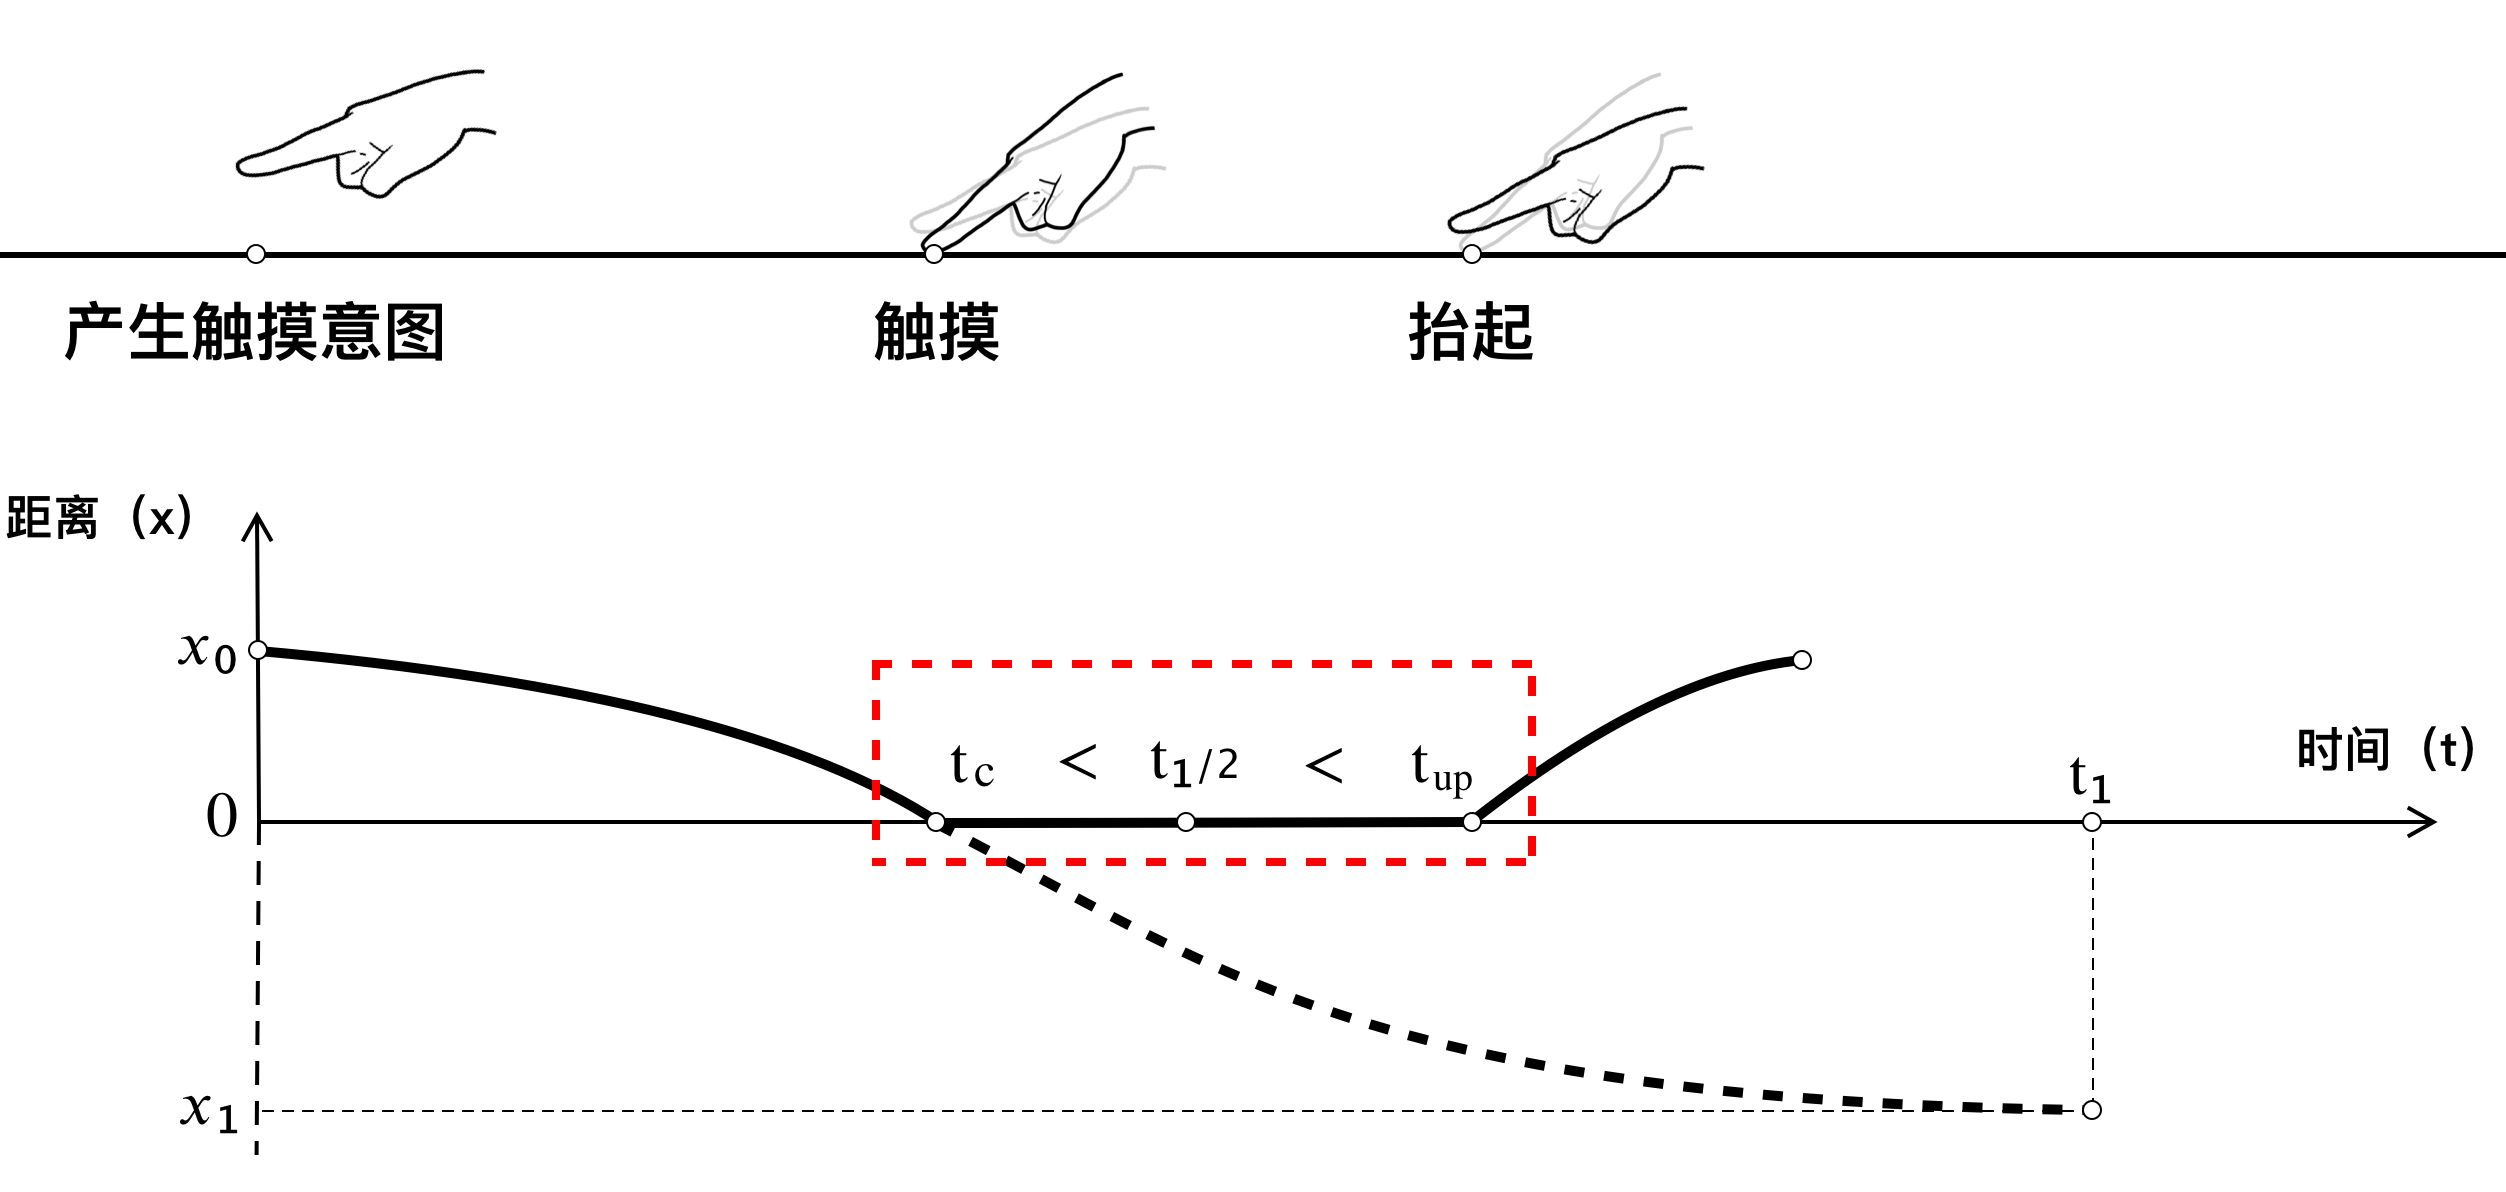
\includegraphics[width=0.8\linewidth]{touch_up_model.png}
	\caption*{触摸运动中点$\frac{t_1}{2}$是触摸运动方程时长的一半,大多数情况下,触摸发生在中点之前,抬起发生在中点之后。}
	\caption{模型为抬起检测提供辅助的判断依据}
	\label{fig:touch_up_model}
\end{figure}

触摸运动模型为抬起检测技术提供了\emph{辅助的判断依据}。如图\ref{fig:touch_up_model}所示,虽然触摸运动模型描述的是触摸前后极短时间内的手指运动规律,并不涉及抬起时的规律,但由于触摸和抬起之间存在相关性,触摸运动模型为抬起检测提供了两点辅助的判断依据:(1)触摸运动中点$\frac{t_1}{2}$是触摸运动方程时长的一半,大多数情况下,触摸发生在中点之前,抬起发生在中点之后;(2)触摸速度与$v(t_c)$与抬起速度$v(t_{up})$之间存在正相关性(R2=0.48)。运用上述两条规律能够提高抬起检测的准确率,从而为触摸手势识别技术奠定基础,本文将在章节\ref{section:model_QwertyRing}中详细介绍触摸和抬起之间的相关性,并介绍触摸手势识别技术。

\subsection{触摸意图推理}

触摸意图推理是判断触摸是否表达交互意图的技术,也称防误触技术。自然触摸交互中人的有意触摸和无意触碰混杂,防误触技术变得重要,同时具有很大的挑战性。本文认为,最佳的防误触技术应从用户意图的层面出发,过滤任何不表达交互意图的触摸。因此,触摸意图的推理是值得研究的问题,而本文所介绍的触摸运动模型为触摸意图推理提供了判断依据。

\subsubsection{基于触摸运动模型的触摸意图推理}

由于有意触摸是用户根据其交互意图刻意组织的,而误触是人在无意识,或者是其意图与当前交互任务无关时造成的,因此有意触摸和误触的触摸运动轨迹应当有所不同。这一规律在触摸运动模型上的体现是,触摸运动方程中的众多参数(如$x_0,x_1, t_1,v(t_c),a(\frac{\tau_1}{2})$),在有意触摸和误触上的分布是不同的:举例来说,通常情况下有意触摸的速度$v(t_c)$更大、意图触摸时长$t_1$更短、手指向下运动时有明显的加速过程(加速度最值$a(\frac{\tau_1}{2})$更大)等等。据此可基于贝叶斯推理,以较大概率区分有意触摸和误触:

\begin{equation}
	\begin{cases}
		P(I) & \propto P(t_1\vert I)P(v(t_c)\vert I)P(a(\frac{\tau_1}{2})\vert I)\cdots \\
		P(\neg I) & \propto P(t_1\vert \neg I)P(v(t_c)\vert I)P(t_1\vert \neg I)P(a(\frac{\tau_1}{2})\vert \neg I)\cdots
	\end{cases}
\end{equation}

其中,$I$表示触摸是有意的,当$P(I)>P(\neg I)$时可判定触摸为有意触摸;当$P(I)<P(\neg I)$时可判定触摸为误触。在理想情况下,$I$或$\neg I$条件概率下触摸运动方程各参数的分布可以通过大量的实验估计得;而对于实际的防误触技术而言,上述式子揭示的现实意义是,触摸运动方程中诸多的参数都可作为触摸意图的判断依据。

\subsubsection{触摸过程与触摸力度之间的关系}

为了验证本文模型为触摸意图推理提供的判据是否实际有效,本章将基于上述思路,实现一种压敏触摸屏平板电脑上的防误触键盘。压敏触摸板所采集的数据是触摸发生以后的触摸面积、触摸压力等数据,而不是触摸运动模型中所涉及的手指位移、速度和加速度信号。在此背景下,若要对触摸运动模型加以利用,就需要探索触摸面积、压力信号与手指运动信号之间的关系,通过压敏触摸板数据间接反映触摸运动方程的参数。

\begin{figure}
	\centering
	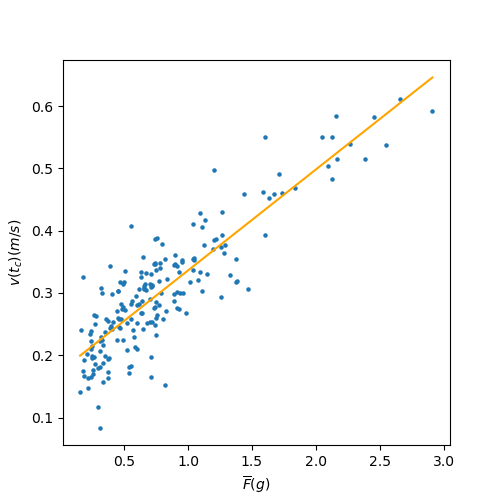
\includegraphics[width=0.6\linewidth]{vdown_vs_F.png}
	\caption*{触摸瞬间手指的运动速度和触摸后手指对交互平面施加的平均压力之间存在正相关的关系。}
	\caption{触摸速度与力度之间的关系}
	\label{fig:vdown_vs_F}
\end{figure}

根据第\ref{section:model}章收集的实验数据,触摸瞬间手指的速度$v(t_c)$与触摸后手指对交互平面施加的平均压力$\overline{F}$之间存在关系:

\begin{equation}
	\overline{F}=0.16\times v(t_c)+0.17
\end{equation}

其中,线性拟合的决定系数(R2)为0.76,也就是说因变量$\overline{F}$的变异中,有76\%的部分可由自变量$v(t_c)$解释。包括平均压力$\overline{F}$在内,研究者发现,压力信号中还有不少特征值可以反映触摸运动方程的参数。例如,触摸瞬间手指速度$v(t_c)$与压力信号的最大值$max(F)$、平均值$\overline{F}$、标准差$\sigma_F$均具有中等程度的相关性($R2=0.65,0.76,0.67$);人产生触摸意图时手指高度$x_0$与$max(F)$、$\overline{F}$、$\sigma_F$均具有弱相关性($R2=0.43,0.58,0.35$);人在组织触摸运动时计划的运动距离$\vert x_1-x_0 \vert$与$\overline{F}$具有弱相关性($R=0.47$);人在组织触摸运动时计划的运动时长$t_1$与手指接触交互表面的总时长$t_{up}-t_c$之间存在弱相关性($R2=0.38$)。上述规律表明,在利用压力信号推理触摸意图的算法中,应该充分发掘压力信号的时空特征,以更好地表征触摸运动状态,从而达到推理触摸意图的目的。

%在这样的拟合程度下,利用触摸运动模型预测触摸力度的精度还不高,但能够粗略地区分轻触和重触,准确率为82.24\%。
%在触摸交互中,人控制触摸力度可用于显示地向计算机表达特定的交互意图\cite{ramos2004pressure, heo2011force, zhong2018forceboard},丰富触摸交互的输入信道;计算机也可以从人触摸的力度大小隐式地推理用户意图\cite{2015-GestureOn},让人机交互更智能。然而,目前还没有商用级别的触摸力度感知算法。触摸运动模型可用于推测触摸力度,这是因为,触摸力度与触摸瞬间手指的运动速度有关,而该运动速度被触摸运动方程所揭示。根据公式\ref{equ:touch_model_v},在触摸瞬间$t_c$手指运动的速度为:

\subsubsection{面向平板电脑键盘的意图推理}

平板电脑键盘上的十指打字是最快速、最复杂的触摸交互任务之一,解决该任务的误触问题对交互效率和体验具有重要意义\cite{gu2021typeboard}。在最理想的防误触能力下,平板电脑应允许用户在打字过程中将非交互手指休息在触摸屏上,而不引发误触,这样一来能大幅缓解用户在长时间打字时面临的疲劳问题。本章后续介绍的实验发现,若用户被允许将手指休息在触摸屏上,多指休息行为导致的无意触碰将占到误触总量的75\%以上,给防误触技术带来很大的挑战。

触摸运动模型能够有效应对上述挑战,有效过滤多指休息行为导致的误触:人在将多根手指休息在触摸屏上时,多根手指的向下运动过程是协同的,因此它们的触摸运动方程参数较为类似。根据这一现象,可利用各手指触摸运动方程的时空相关性来识别多指休息行为,从而将多指休息行为导致的触摸事件判定为误触。



\section{本章小结}

本章提出了基于最优控制理论的触摸运动模型。最优控制理论与神经系统的学科交叉\cite{flash1985coordination}指出,人的肢体运动倾向于最小化其急动度的平方积分,在此假设下,本章推导出触摸运动模型的数学表达,即触摸运动过程是一个分段的五次函数(公式\ref{equ:touch_model})。进一步地,本章提出了触摸运动模型的计算方法,即使用卡尔曼滤波和最小二乘法来拟合触摸运动方程参数。最后,本章通过实验验证了触摸运动模型的合理性,也表明了触摸运动方程是对触摸运动过程的良好拟合。在本文接下来的三章中,将介绍触摸运动模型在三种典型的触摸交互技术中的应用。
